\documentclass[11pt,a4paper]{article}
\usepackage[margin=2.2cm]{geometry}
\usepackage{amsmath,amssymb,bm}
\usepackage{booktabs}
\usepackage{tabularx}
\usepackage{listings}
\usepackage{xcolor}
\usepackage{hyperref}
\usepackage{tikz}
\usepackage{pgfplots}
\pgfplotsset{compat=1.18}
\usetikzlibrary{positioning,arrows.meta,calc,shapes.geometric,decorations.pathreplacing,decorations.pathmorphing,fit,backgrounds,patterns}
\usepackage{enumitem}
\usepackage{array}
\usepackage{float}
\usepackage{caption}
\usepackage{fancyhdr}
\usepackage{graphicx}
\usepackage[most]{tcolorbox}

% ============================================================================
% COLOUR PALETTE
% ============================================================================
\definecolor{hwblue}{RGB}{20,80,160}
\definecolor{phase1green}{RGB}{30,130,60}
\definecolor{phase2orange}{RGB}{200,100,20}
\definecolor{exopurple}{RGB}{120,40,170}
\definecolor{warnbar}{RGB}{200,140,0}
\definecolor{resultbar}{RGB}{40,140,60}
\definecolor{resultbg}{RGB}{230,255,230}
\definecolor{warnbg}{RGB}{255,245,220}
\definecolor{pybg}{RGB}{248,252,248}
\definecolor{pyframe}{RGB}{160,190,160}
\definecolor{pykw}{RGB}{0,110,0}
\definecolor{pycmt}{RGB}{100,100,100}
\definecolor{pystr}{RGB}{160,32,240}

% ============================================================================
% TCOLORBOX ENVIRONMENTS
% ============================================================================
\newtcolorbox{resultbox}[1][]{enhanced,breakable,
  colback=resultbg,colframe=resultbar,boxrule=0.6pt,
  left=4pt,right=4pt,top=4pt,bottom=4pt,
  title={\textcolor{resultbar}{\sffamily\bfseries{\large$\checkmark$}~Key Result} #1},
  attach boxed title to top left={yshift=-2mm,xshift=4mm},
  boxed title style={colback=resultbg,colframe=resultbar}}

\newtcolorbox{warnbox}[1][]{enhanced,breakable,
  colback=warnbg,colframe=warnbar,boxrule=0.6pt,
  left=4pt,right=4pt,top=4pt,bottom=4pt,
  title={\textcolor{warnbar}{\sffamily\bfseries{\large$\triangle$}~Important} #1},
  attach boxed title to top left={yshift=-2mm,xshift=4mm},
  boxed title style={colback=warnbg,colframe=warnbar}}

\newtcolorbox{archbox}[1][]{enhanced,breakable,
  colback=blue!3,colframe=hwblue,boxrule=0.6pt,
  left=4pt,right=4pt,top=4pt,bottom=4pt,
  title={\textcolor{hwblue}{\sffamily\bfseries #1}},
  attach boxed title to top left={yshift=-2mm,xshift=4mm},
  boxed title style={colback=blue!3,colframe=hwblue}}

\newtcolorbox{phase1box}[1][]{enhanced,breakable,
  colback=green!4,colframe=phase1green,boxrule=0.8pt,
  left=4pt,right=4pt,top=4pt,bottom=4pt,
  title={\textcolor{phase1green}{\sffamily\bfseries{\large$\bigstar$}~Phase~1: #1}},
  attach boxed title to top left={yshift=-2mm,xshift=4mm},
  boxed title style={colback=green!4,colframe=phase1green}}

\newtcolorbox{phase2box}[1][]{enhanced,breakable,
  colback=orange!4,colframe=phase2orange,boxrule=0.8pt,
  left=4pt,right=4pt,top=4pt,bottom=4pt,
  title={\textcolor{phase2orange}{\sffamily\bfseries{\large$\bigstar$}~Phase~2: #1}},
  attach boxed title to top left={yshift=-2mm,xshift=4mm},
  boxed title style={colback=orange!4,colframe=phase2orange}}

\newtcolorbox{exobox}[1][]{enhanced,breakable,
  colback=violet!4,colframe=exopurple,boxrule=0.6pt,
  left=4pt,right=4pt,top=4pt,bottom=4pt,
  title={\textcolor{exopurple}{\sffamily\bfseries #1}},
  attach boxed title to top left={yshift=-2mm,xshift=4mm},
  boxed title style={colback=violet!4,colframe=exopurple}}

\newtcolorbox{lecturebox}[1][]{enhanced,breakable,
  colback=hwblue!3,colframe=hwblue,boxrule=0.8pt,
  left=4pt,right=4pt,top=4pt,bottom=4pt,
  title={\textcolor{hwblue}{\sffamily\bfseries\large Lecture Focus} #1},
  attach boxed title to top left={yshift=-2mm,xshift=4mm},
  boxed title style={colback=hwblue!3,colframe=hwblue}}

% ============================================================================
% LISTINGS
% ============================================================================
\lstset{
  language=Python,
  basicstyle=\ttfamily\small,
  keywordstyle=\color{pykw}\bfseries,
  commentstyle=\color{pycmt}\itshape,
  stringstyle=\color{pystr},
  numbers=left, numberstyle=\tiny\color{gray},
  frame=single, breaklines=true, columns=fullflexible,
  showstringspaces=false,
  backgroundcolor=\color{pybg},
  morekeywords={np,self,True,False,None,float},
}

% ============================================================================
% HEADER / FOOTER
% ============================================================================
\pagestyle{fancy}
\fancyhf{}
\fancyhead[L]{\small\textcolor{hwblue}{\textbf{4-Actuator Exo-Arm --- Trajectory Control \& Hardware}}}
\fancyhead[R]{\small\textcolor{gray}{exo-actuator-sensor-drivers}}
\fancyfoot[C]{\thepage}
\renewcommand{\headrulewidth}{0.5pt}
\renewcommand{\headrule}{\hbox to\headwidth{\color{hwblue}\leaders\hrule height \headrulewidth\hfill}}

% ============================================================================
% MACROS
% ============================================================================
\newcommand{\vq}{\bm{q}}
\newcommand{\vqd}{\dot{\bm{q}}}
\newcommand{\vqdd}{\ddot{\bm{q}}}
\newcommand{\vtau}{\bm{\tau}}
\newcommand{\vp}{\bm{p}}
\newcommand{\vpd}{\dot{\bm{p}}}
\newcommand{\vpdd}{\ddot{\bm{p}}}
\newcommand{\ve}{\bm{e}}
\newcommand{\ved}{\dot{\bm{e}}}
\newcommand{\M}{\bm{M}}
\newcommand{\Cor}{\bm{C}}
\newcommand{\vg}{\bm{g}}
\newcommand{\J}{\bm{J}}
\newcommand{\Kp}{\bm{K}_p}
\newcommand{\Kd}{\bm{K}_d}
\newcommand{\Ki}{\bm{K}_i}
\newcommand{\diag}{\operatorname{diag}}
\newcommand{\rp}{r_{\mathrm{p}}}
\newcommand{\ks}{k_{\mathrm{s}}}
\newcommand{\bc}{b_{\mathrm{c}}}
\newcommand{\lm}{l_{\mathrm{m}}}
\newcommand{\lmd}{\dot{l}_{\mathrm{m}}}

% ============================================================================
\title{%
  \textcolor{hwblue}{\rule{\linewidth}{1.5pt}}\\[0.4cm]
  {\LARGE\bfseries 4-Actuator Exo-Arm System}\\[0.3cm]
  {\large Trajectory Control: from Simple Hardware PD\\to Model-Based Computed Torque}\\[0.2cm]
  {\normalsize AK80-kv60 (shoulder)\,$\cdot$\,AK60-kv80 (elbow)\,$\cdot$\,
   2$\times$ Damiao (exo)\,$\cdot$\,AS5048A encoder}\\[0.4cm]
  \textcolor{hwblue}{\rule{\linewidth}{1.5pt}}
}
\author{Repo \texttt{exo-actuator-sensor-drivers}}
\date{May 2026}
% ============================================================================

\begin{document}
\maketitle\thispagestyle{empty}

% ------- Key results -------------------------------------------------------
\begin{resultbox}
\begin{itemize}[leftmargin=1.5em]
  \item \textbf{Phase 1 (start here):} MIT on-board PD requires \emph{no mass/CoM knowledge}.
        Shoulder and elbow track joint-space references; exo Damiao motors hold
        transparent (zero-torque) mode.  AS5048A provides accurate absolute
        elbow angle independent of CAN round-trip latency.
  \item \textbf{Phase 2 (after identification):} Computed-Torque inversion of the
        full nonlinear dynamics cancels inertia and Coriolis coupling (gravity
        is negligible: arm moves in the horizontal XY plane, gravity acts in $-Z$).  Series
        Elastic Actuator (SEA) compensation at the elbow accounts for cable-spring
        lag between motor drum position and joint angle.
\end{itemize}
\end{resultbox}

\tableofcontents
\newpage

\begin{figure}[H]
\centering
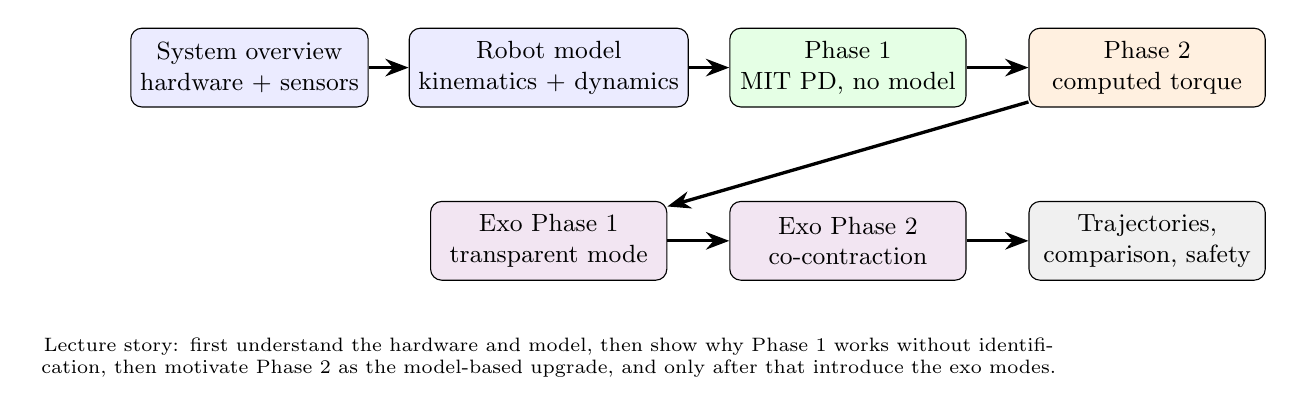
\begin{tikzpicture}[>=Stealth, every node/.style={font=\small, align=center}]
  \def\bw{3.0cm}
  \def\bh{1.0cm}

  \node[draw, rounded corners=4pt, fill=blue!8,
        minimum width=\bw, minimum height=\bh] (sys)
      at (0,0) {System overview\\hardware + sensors};
  \node[draw, rounded corners=4pt, fill=blue!8,
        minimum width=\bw, minimum height=\bh] (model)
      at (3.8,0) {Robot model\\kinematics + dynamics};
  \node[draw, rounded corners=4pt, fill=green!10,
        minimum width=\bw, minimum height=\bh] (p1)
      at (7.6,0) {Phase 1\\MIT PD, no model};
  \node[draw, rounded corners=4pt, fill=orange!12,
        minimum width=\bw, minimum height=\bh] (p2)
      at (11.4,0) {Phase 2\\computed torque};

  \node[draw, rounded corners=4pt, fill=violet!10,
        minimum width=\bw, minimum height=\bh] (exo1)
      at (3.8,-2.2) {Exo Phase 1\\transparent mode};
  \node[draw, rounded corners=4pt, fill=violet!10,
        minimum width=\bw, minimum height=\bh] (exo2)
      at (7.6,-2.2) {Exo Phase 2\\co-contraction};
  \node[draw, rounded corners=4pt, fill=gray!12,
        minimum width=\bw, minimum height=\bh] (traj)
      at (11.4,-2.2) {Trajectories,\\comparison, safety};

  \draw[->, very thick] (sys) -- (model);
  \draw[->, very thick] (model) -- (p1);
  \draw[->, very thick] (p1) -- (p2);
  \draw[->, very thick] (p2) -- (exo1);
  \draw[->, very thick] (exo1) -- (exo2);
  \draw[->, very thick] (exo2) -- (traj);

  \node[font=\scriptsize, text width=13cm, below=0.6cm of exo1]
      {Lecture story: first understand the hardware and model, then show why Phase~1 works without identification, then motivate Phase~2 as the model-based upgrade, and only after that introduce the exo modes.};
\end{tikzpicture}
\caption{Lecture roadmap for the printed notes. This gives the audience a high-level map of the narrative before the technical details begin.}
\label{fig:lecture_roadmap}
\end{figure}

% =========================================================================
\section{System Overview}
\label{sec:system}
% =========================================================================

The bench robot is a \textbf{2-DOF planar arm} with two joints:
\begin{itemize}[leftmargin=2em]
  \item \textbf{Shoulder ($q_1$) — direct drive.}  AK80-kv60 motor is
        \emph{housed inside the 3D-printed base housing}.  Its output shaft
        connects directly to Link~1; there is no cable between the motor and
        the link.
  \item \textbf{Elbow ($q_2$) — cable SEA.}  AK60-kv80 motor is
        \emph{mounted on Link~1} (near the elbow end, inside the link
        structure) and drives the joint through two antagonistic cables.
        The cables route from the motor drum through 623zz idler bearings
        along Link~1 and wrap around the \textbf{elbow joint drum} ($r_p{=}47.75$\,mm)
        fixed on the elbow shaft.  A spring element $k_s$ on the cable forms a
        Series Elastic Actuator (SEA).
\end{itemize}
One \textbf{Damiao} motor (\emph{second not yet mounted}) adds an
\textbf{exo cable} to the elbow joint drum, providing additional
stiffness when activated.
An \textbf{AS5048A} absolute magnetic encoder on the elbow joint axis reads
the true joint angle, bypassing the cable-spring deflection that corrupts
the motor's CAN feedback.

\subsection{Hardware inventory}

\begin{center}\small
\begin{tabular}{llllll}
\toprule
\textbf{Joint} & \textbf{Motor} & \textbf{Firmware} & \textbf{Driver file} & $T_{\max}$ & \textbf{Notes} \\
\midrule
Shoulder ($q_1$) & CubeMars AK80-kv60  & V1.x & \texttt{ak\_v1\_bus.py} & 32\,N$\cdot$m & \textbf{Direct drive}; inside base housing; std 11-bit CAN \\
Elbow ($q_2$)    & CubeMars AK60-kv80  & V3.0 & \texttt{ak\_v3\_bus.py} & 15\,N$\cdot$m & \textbf{Cable SEA}; mounted on Link~1; ext 29-bit CAN \\
Exo ($\theta_{e}$) & Damiao DM4310 & MIT  & \texttt{damiao\_bus.py} & 10\,N$\cdot$m & 1 motor mounted; \texttt{can\_id=0x01}; 2nd not yet fitted \\
Elbow encoder & AS5048A (14-bit SPI) & --- & \texttt{as5048a.py} & --- & \texttt{/dev/spidev0.0} (Jetson Orin) \\
Elbow encoder & AS5048A (14-bit SPI) & --- & \texttt{as5048a.py} & --- & \texttt{/dev/spidev0.0} (Jetson Orin) \\
\bottomrule
\end{tabular}
\end{center}

\begin{warnbox}
\textbf{Two CAN firmwares on one bus.}
AK80-kv60 (shoulder) uses V1.x firmware with \textbf{standard 11-bit CAN frames};
AK60-kv80 (elbow) uses V3.0 firmware with \textbf{29-bit extended frames}.
Both can coexist on \texttt{can1} because CAN hardware distinguishes frame
types, but they require \emph{separate} bus wrapper objects
(\texttt{CubeMarsAkV1Bench} vs.\ \texttt{CubeMarsAkV3Bench}).
\end{warnbox}

\subsection{Geometric and physical parameters}

\begin{center}\small
\begin{tabular}{llll}
\toprule
Symbol & Meaning & Simulation value (Onshape URDF) & Hardware (TBD) \\
\midrule
$L_1$      & Upper-arm link length          & 335\,mm & measure \\
$L_2$      & Forearm link length            & 380\,mm & measure \\
$m_1$      & Upper-arm mass (incl.\ motor)  & 5.313\,kg & weigh \\
$m_2$      & Forearm mass (incl.\ motor)    & 0.764\,kg & weigh \\
$l_{c1}$   & Upper-arm CoM distance         & $L_1/2$ (rod approx.) & balance \\
$l_{c2}$   & Forearm CoM distance           & $L_2/2$ (rod approx.) & balance \\
$\rp$      & Drum radius (motor output shaft \& elbow joint shaft)  & 47.75\,mm & measure \\
$r_{\mathrm{exo}}$ & Exo elbow drum radius (same drum as drive cable) & 47.75\,mm & measure \\
\bottomrule
\end{tabular}
\end{center}

% ─────────────────────────────────────────────────────────────────────────────
\subsection{Mechanical structure and cable routing}
\label{sec:mech}
% ─────────────────────────────────────────────────────────────────────────────

\begin{figure}[H]
\centering
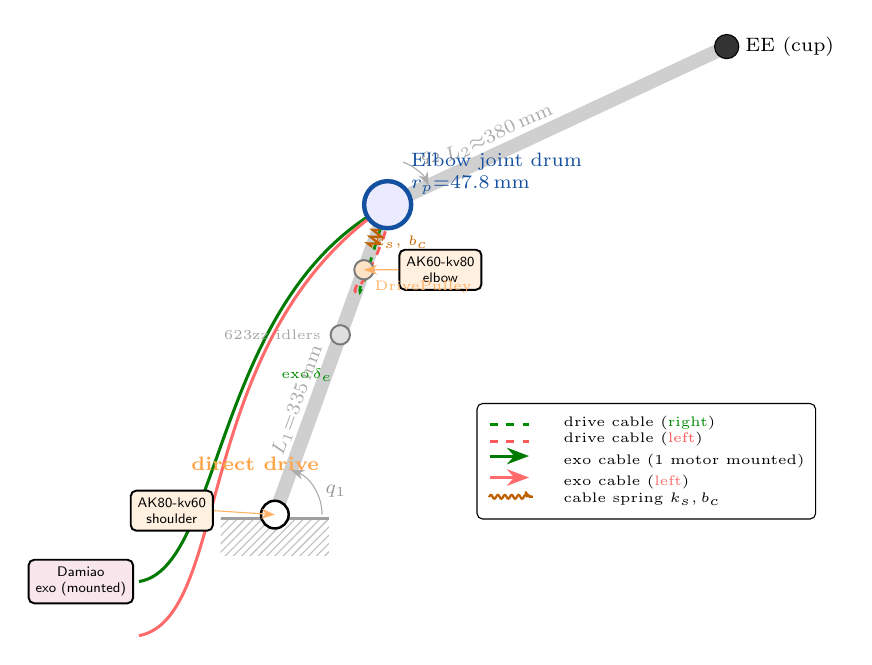
\begin{tikzpicture}[>=Stealth, scale=1.25,
  %% styles
  link/.style    ={line width=5pt, gray!38, line cap=round},
  jcirc/.style   ={circle, draw=black, fill=white, line width=0.9pt,
                   inner sep=0pt, minimum size=10pt},
  bigp/.style    ={circle, draw=hwblue, fill=blue!8, line width=1.6pt,
                   inner sep=0pt, minimum size=17pt},
  smallp/.style  ={circle, draw=darkgray!70, fill=gray!25, line width=0.7pt,
                   inner sep=0pt, minimum size=7pt},
  mbox/.style    ={draw, rounded corners=2pt, fill=orange!12, font=\tiny\sffamily,
                   align=center, inner sep=2.5pt, line width=0.7pt},
  dbox/.style    ={draw, rounded corners=2pt, fill=purple!10, font=\tiny\sffamily,
                   align=center, inner sep=2.5pt, line width=0.7pt},
  ann/.style     ={font=\scriptsize},
]
  %% ── Arm keypoints  (1 unit = 100 mm) ──────────────────────────────────
  %% q1 = 70° (from horizontal);  |L1| = 3.35;  link2 direction = 25° abs
  \coordinate (SH) at (0.000, 0.000);   %% shoulder joint
  \coordinate (EL) at (1.146, 3.148);   %% elbow joint  (BigPulley on link2)
  \coordinate (EE) at (4.590, 4.754);   %% end-effector
  \coordinate (DP) at (0.905, 2.487);   %% DrivePulley  (79\% along link1)
  \coordinate (ID) at (0.665, 1.826);   %% 623zz idler  (58\% along link1)

  %% ── Ground ─────────────────────────────────────────────────────────────
  \fill[pattern=north east lines, pattern color=gray!50]
      (-0.55,-0.42) rectangle (0.55,-0.04);
  \draw[thick, gray!75] (-0.55,-0.04) -- (0.55,-0.04);

  %% ── Link bodies ────────────────────────────────────────────────────────
  \draw[link] (SH) -- (EL);   %% Link 1 (upper arm)
  \draw[link] (EL) -- (EE);   %% Link 2 (forearm)

  %% ── Drive cables (two antagonistic, from DrivePulley → idler → BigPulley)
  %% green cable (right, pulls link2 in +q2 direction)
  \draw[green!55!black, line width=1.0pt, dashed]
      (DP)
      .. controls ($(ID)+(0.09, 0.00)$) and ($(EL)+(-0.10,-0.32)$)
      .. (EL);
  %% red cable (left, pulls link2 in -q2 direction)
  \draw[red!65, line width=1.0pt, dashed]
      (DP)
      .. controls ($(ID)+(-0.09, 0.00)$) and ($(EL)+(0.10,-0.32)$)
      .. (EL);
  %% spring symbol (SEA) midway along the drive cable, offset to the right
  \draw[decorate,
        decoration={zigzag, segment length=2.6pt, amplitude=2pt},
        orange!75!black, line width=0.8pt]
      ($(DP)!0.35!(EL)$) -- ($(DP)!0.65!(EL)$);
  \node[ann, orange!80!black] at (1.28, 2.77)
      {\tiny $k_s,\,b_c$};

  %% ── Exo cables (from Damiao motors at base → BigPulley) ────────────────
  \draw[green!48!black, line width=1.1pt, -Stealth]
      (-1.38,-0.68)
      .. controls (-0.55,-0.55) and (-0.62, 2.10)
      .. (EL);
  \draw[red!58, line width=1.1pt, -Stealth]
      (-1.38,-1.23)
      .. controls (-0.45,-1.05) and (-0.85, 1.70)
      .. (EL);

  %% ── Pulley symbols ──────────────────────────────────────────────────────
  \node[smallp, fill=orange!22] at (DP) {};    %% DrivePulley
  \node[smallp]                 at (ID) {};    %% 623zz idler
  \node[bigp]                   at (EL) {};    %% BigPulley (elbow joint)

  %% ── Joints ──────────────────────────────────────────────────────────────
  \node[jcirc] at (SH) {};

  %% ── End-effector ────────────────────────────────────────────────────────
  \filldraw[fill=black!80, draw=black] (EE) circle (3.5pt);

  %% ── Motor boxes ─────────────────────────────────────────────────────────
  \node[mbox, anchor=east] (MS) at (-0.62, 0.04)
      {AK80-kv60\\shoulder};
  \draw[-Stealth, thin, orange!60] (MS.east) -- (SH);
  \node[ann, orange!70, font=\scriptsize\bfseries] at (-0.20, 0.52)
      {direct drive};

  \node[mbox, anchor=west] (ME) at ($(DP)+(0.35,0)$)
      {AK60-kv80\\elbow};
  \draw[-Stealth, thin, orange!60] (ME.west) -- (DP);
  \node[ann, orange!60, anchor=west, font=\tiny] at ($(DP)+(0.01,-0.18)$)
      {DrivePulley};

  \node[dbox, anchor=east] (MDR) at (-1.43,-0.68)
      {Damiao\\exo (mounted)};

  %% ── Joint angle arcs ────────────────────────────────────────────────────
  \draw[->, gray!65, thin] ($(SH)+(0.48,0)$) arc (0:70:0.48);
  \node[ann, gray!80] at ($(SH)+(0.62,0.24)$) {$q_1$};

  \draw[->, gray!65, thin] ($(EL)+(70:0.46)$) arc (70:25:0.46);
  \node[ann, gray!80] at ($(EL)+(47:0.65)$) {$q_2$};

  %% ── Link length labels ──────────────────────────────────────────────────
  \node[ann, gray!65, rotate=70, anchor=south] at ($(SH)!0.35!(EL)$)
      {$L_1{=}335\,\mathrm{mm}$};
  \node[ann, gray!65, rotate=25, anchor=south] at ($(EL)!0.35!(EE)$)
      {$L_2{\approx}380\,\mathrm{mm}$};

  %% ── BigPulley label ─────────────────────────────────────────────────────
  \node[ann, hwblue, anchor=west, align=left] at ($(EL)+(0.14,0.32)$)
      {Elbow joint drum\\$r_p{=}47.8\,\mathrm{mm}$};

  %% ── 623zz idler label ───────────────────────────────────────────────────
  \node[ann, gray!70, anchor=east] at ($(ID)+(-0.10,0)$)
      {\tiny 623zz idlers};

  %% ── Exo cable labels ────────────────────────────────────────────────────
  \node[ann, green!55!black, anchor=west, font=\tiny] at (-0.03, 1.42)
      {exo\,$\delta_e$};

  %% ── EE label ────────────────────────────────────────────────────────────
  \node[ann, anchor=west] at ($(EE)+(0.09,0)$) {EE (cup)};

  %% ── Legend ──────────────────────────────────────────────────────────────
  \node[draw, fill=white, rounded corners=2pt, inner sep=4pt,
        anchor=south east, font=\tiny]
      at (5.5, -0.05) {
      \begin{tabular}{@{}ll@{}}
        \tikz\draw[green!55!black,dashed,line width=1pt](0,0)--(0.5cm,0); &
            drive cable (\textcolor{green!55!black}{right}) \\
        \tikz\draw[red!65,dashed,line width=1pt](0,0)--(0.5cm,0); &
            drive cable (\textcolor{red!65}{left}) \\
        \tikz\draw[green!48!black,-Stealth,line width=1.1pt](0,0)--(0.5cm,0); &
            exo cable (1 motor mounted) \\
        \tikz\draw[red!58,-Stealth,line width=1.1pt](0,0)--(0.5cm,0); &
            exo cable (\textcolor{red!58}{left}) \\
        \tikz\draw[decorate,decoration={zigzag,segment length=2.5pt,amplitude=1.8pt},orange!75!black,line width=0.8pt](0,0)--(0.5cm,0); &
            cable spring $k_s,b_c$ \\
      \end{tabular}
  };
\end{tikzpicture}
\caption{%
  Mechanical structure of the 4-actuator arm (canonical pose: $q_1{=}70^\circ$, $q_2{=}{-}45^\circ$).
  \textbf{Shoulder joint~$q_1$}: direct-drive AK80-kv60 at the base.
  \textbf{Elbow joint~$q_2$}: cable-driven via two antagonistic cables.
  The AK60-kv80 elbow motor (mounted on Link~1, near the elbow end at $\sim\!79\%$ of $L_1$,
  inside the link structure) drives a motor drum; cables pass over 623zz idler bearings and wrap around
  the elbow joint drum ($r_p{=}47.8$\,mm) on the elbow shaft.  A zigzag symbol marks the cable
  spring $k_s,b_c$ (SEA).  One Damiao exo motor (second not yet mounted)
  delivers an exo cable to the elbow joint drum.  Both CubeMars motors are enclosed
  inside the 3D-printed arm structure and are not externally visible.
}
\label{fig:mech}
\end{figure}

\subsection{Multi-bus topology}

\begin{archbox}{4-Actuator Bus Architecture}
\begin{center}
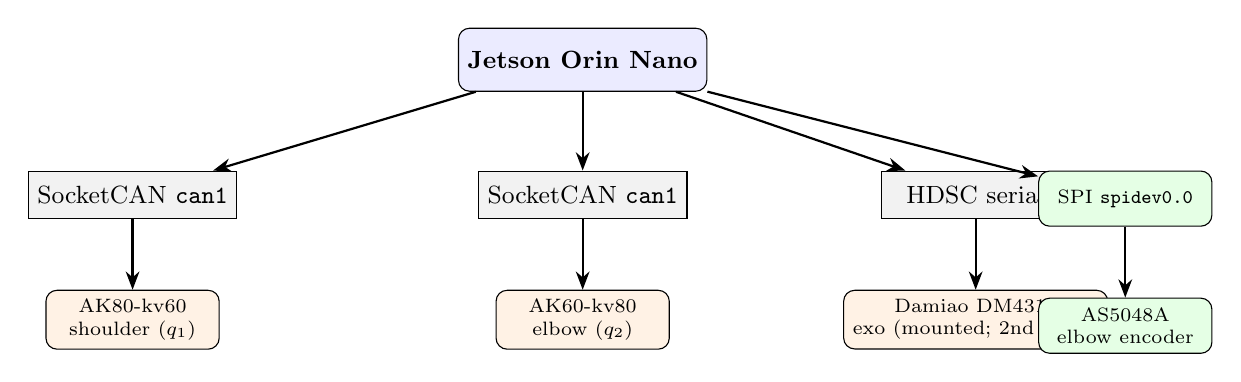
\begin{tikzpicture}[
  >=Stealth,
  host/.style={draw,rounded corners,fill=blue!8,font=\small\bfseries,
               minimum width=3.0cm,minimum height=0.8cm},
  bus/.style={draw,fill=gray!10,font=\small,
              minimum width=2.4cm,minimum height=0.6cm},
  motor/.style={draw,rounded corners,fill=orange!10,font=\scriptsize,
                minimum width=2.2cm,minimum height=0.7cm,align=center},
  enc/.style={draw,rounded corners,fill=green!10,font=\scriptsize,
              minimum width=2.2cm,minimum height=0.7cm,align=center},
  arr/.style={-Stealth,thick},
]
  \node[host] (host) {Jetson Orin Nano};

  \node[bus,below left=1.0cm and 2.8cm of host]  (v1can)  {SocketCAN \texttt{can1}};
  \node[bus,below=1.0cm of host]                  (v3can)  {SocketCAN \texttt{can1}};
  \node[bus,below right=1.0cm and 2.2cm of host]  (serial) {HDSC serial};
  \node[enc,below right=1.0cm and -0.8cm of host, xshift=5.0cm] (spi) {SPI \texttt{spidev0.0}};

  \node[motor,below=0.9cm of v1can]  (ak80) {AK80-kv60\\shoulder ($q_1$)};
  \node[motor,below=0.9cm of v3can]  (ak60) {AK60-kv80\\elbow ($q_2$)};
  \node[motor,below=0.9cm of serial]  (dm1)  {Damiao DM4310\\exo (mounted; 2nd TBD)};
  \node[enc,below=0.9cm of spi]      (enc)  {AS5048A\\elbow encoder};

  \draw[arr] (host) -- (v1can);
  \draw[arr] (host) -- (v3can);
  \draw[arr] (host) -- (serial);
  \draw[arr] (host) -- (spi);
  \draw[arr] (v1can)  -- (ak80);
  \draw[arr] (v3can)  -- (ak60);
  \draw[arr] (serial) -- (dm1);
  \draw[arr] (spi)    -- (enc);
\end{tikzpicture}
\end{center}
\end{archbox}

\begin{lstlisting}[caption={Bus instantiation using declarative configs (\texttt{src/motor\_config.py}).}]
from motor_config import (
    CubeMarsAkV1BusConfig, CubeMarsAkV1MotorConfig,   # shoulder
    CubeMarsAkV3BusConfig, CubeMarsMotorConfig,        # elbow
    DamiaoBusConfig,        DamiaoMotorConfig,         # exo
)
from encoder_config import AS5048AConfig

# Shoulder: AK80-kv60  (V1.x, standard CAN frames)
shoulder_cfg = CubeMarsAkV1BusConfig(
    channel="can1",
    motors={"shoulder": CubeMarsAkV1MotorConfig(can_id=0x01, model="AK80-8")},
)

# Elbow: AK60-kv80  (V3.0, extended CAN frames)
elbow_cfg = CubeMarsAkV3BusConfig(
    channel="can1",
    motors={"elbow": CubeMarsMotorConfig(can_id=0x02, model="AK60-6")},
)

# Exo: 1x Damiao DM4310 mounted (2nd not yet installed)
exo_cfg = DamiaoBusConfig(
    port="/dev/ttyACM0",
    motors={
        "exo": DamiaoMotorConfig(can_id=0x01, master_id=0x11),
    },
)

# Elbow absolute encoder: AS5048A (SPI bus 0, CS 0)
enc_cfg = AS5048AConfig(bus=0, device=0, max_hz=1_000_000)
\end{lstlisting}

% =========================================================================
\section{Robot Model (Reference for Phase 2)}
\label{sec:model}
% =========================================================================

\textbf{Phase~1 does not use any of this section.}
Skip ahead to Section~\ref{sec:phase1} for commissioning.
Phase~2 requires the physical parameters in the table above.

\subsection{Forward kinematics}

Let $s_1{=}\sin q_1$, $c_1{=}\cos q_1$,
$s_{12}{=}\sin(q_1{+}q_2)$, $c_{12}{=}\cos(q_1{+}q_2)$:
\begin{equation}
  \vp(\vq) = \begin{bmatrix} x \\ y \end{bmatrix}
           = \begin{bmatrix}
               L_1 c_1 + L_2 c_{12} \\
               L_1 s_1 + L_2 s_{12}
             \end{bmatrix}.
  \label{eq:fk}
\end{equation}

\subsection{Jacobian}

$\vpd = \J(\vq)\,\vqd$, where
\begin{equation}
  \J(\vq) = \begin{bmatrix}
    -L_1 s_1 - L_2 s_{12} & -L_2 s_{12} \\
     L_1 c_1 + L_2 c_{12} &  L_2 c_{12}
  \end{bmatrix}.
  \label{eq:jac}
\end{equation}
Damped pseudoinverse $\J^\dagger{=}\J^T(\J\J^T+\lambda^2\mathbf{I})^{-1}$
is used near singularities ($\lambda{\approx}0.01$).

\subsection{Equations of motion}

\begin{equation}
  \M(\vq)\,\vqdd + \Cor(\vq,\vqd)\,\vqd + \vg(\vq) = \vtau.
  \label{eq:eom}
\end{equation}

\paragraph{Inertia matrix} (uniform-rod model, $c_2{=}\cos q_2$):
\begin{align}
  M_{11} &= \tfrac{4}{3}m_1 L_1^2 + m_2(L_1^2 + \tfrac{4}{3}L_2^2 + 2L_1 L_2 c_2),\notag\\
  M_{12} &= m_2(\tfrac{4}{3}L_2^2 + L_1 L_2 c_2),\quad
  M_{22}  = \tfrac{4}{3}m_2 L_2^2.
  \label{eq:M}
\end{align}

\paragraph{Coriolis/centrifugal} ($h{=}{-}m_2 L_1 L_2 s_2$):
\begin{equation}
  \Cor = \begin{bmatrix}h\dot{q}_2 & h(\dot{q}_1{+}\dot{q}_2)\\
                        -h\dot{q}_1 & 0\end{bmatrix}.
  \label{eq:C}
\end{equation}

\paragraph{Gravity.}
The arm moves in the horizontal $XY$ plane; gravity acts in $-Z$ (perpendicular
to the plane of motion).  Because no link rotation occurs about a horizontal
axis, gravity produces \textbf{no torque on either joint}:
\begin{equation}
  \vg(\vq) = \mathbf{0}.
  \label{eq:grav}
\end{equation}
This simplifies the equations of motion and the Computed-Torque law: the
$\vg(\vq)$ term vanishes, leaving only inertia and Coriolis effects to cancel.

\subsection{Inverse kinematics}

\begin{equation}
  q_2 = \operatorname{atan2}\!\Bigl(\pm\sqrt{1-D^2},\;D\Bigr),\quad
  D = \frac{x^2+y^2-L_1^2-L_2^2}{2L_1 L_2},
  \label{eq:ik}
\end{equation}
\begin{equation}
  q_1 = \operatorname{atan2}(y,x) - \operatorname{atan2}(L_2 s_2,\;L_1+L_2 c_2).
\end{equation}

% =========================================================================
\section{Cable Transmission Model}
\label{sec:cable}
% =========================================================================

This section describes the cable mechanics for the elbow SEA drive and exo cables.
\textbf{Joint~1 (shoulder) torque passes through unchanged}; all cable
dynamics apply to joint~2 (elbow) only.

\subsection{Drive cable (SEA on elbow, joint 2)}
\label{sec:sea_model}

The AK60-kv80 motor drives \textbf{two antagonistic cables}.  Each cable
wraps on a \textbf{motor drum} fixed to the motor output shaft
(radius~$\rp = 47.75$\,mm).  The other end wraps on the
\textbf{elbow joint drum} fixed to the elbow shaft (same radius~$\rp$),
so one full revolution of the motor output shaft reels in $2\pi\rp$ of
cable.  Both cables are wound in opposite directions, making the drive
\emph{antagonistic}: winding one cable slackens the other.

\begin{warnbox}
\textbf{Only one cable is ever taut at a time.}
Both cables are wound on the motor drum in opposite directions.  When the
motor output shaft rotates in the $+$ direction it \emph{winds} the green
cable (shortening
it $\to$ tension) and simultaneously \emph{unwinds} the red cable
(lengthening it $\to$ slack).  The reverse is true for the $-$ direction.
The two cables therefore \emph{cannot} both be taut simultaneously ---
whichever side is slack carries zero force.  The spring $k_s$ is in series
with each cable, so ``spring extension'' $\delta$ is purely a signed scalar:
$\delta > 0$ means green cable is loaded; $\delta < 0$ means red cable is
loaded.
\end{warnbox}

Choosing motor-side cable displacement as state, with drum radius
$\rp = 47.75$\,mm (both drums — motor output shaft and elbow joint shaft):

\paragraph{Cable extension (spring deflection):}
\begin{equation}
  \delta = \rp\,\theta_m - \rp\,q_2
         = \rp(\theta_m - q_2).
  \label{eq:delta_drive}
\end{equation}
$\delta > 0$: green cable is shortened (taut); red cable is slack.\\
$\delta < 0$: red cable is shortened (taut); green cable is slack.\\
In \textbf{position mode} the state is the cable displacement
$\lm = \rp\,\theta_m$, giving $\delta = \lm - \rp\,q_2$.

\paragraph{Cable force (unilateral spring–damper):}

Because cables can only pull, the raw spring force is split into the active
cable's tension and the slack cable contributes nothing:
\begin{equation}
  F_{\mathrm{raw}} = \ks\,\delta + \bc\,\dot{\delta}.
  \label{eq:fraw}
\end{equation}
\begin{align}
  T_{\mathrm{green}} &= \max(F_{\mathrm{raw}},\;0),\quad
  T_{\mathrm{red}}   = \max(-F_{\mathrm{raw}},\;0).
  \label{eq:unilateral}
\end{align}

At any instant $T_{\mathrm{green}}\cdot T_{\mathrm{red}} = 0$: \emph{exactly
one} of the two is non-zero (or both are zero at $\delta = 0$, i.e.\ no load).
The net cable force on the elbow joint drum is
$F_{\mathrm{cable}} = T_{\mathrm{green}} - T_{\mathrm{red}}$.

\paragraph{Joint torque:}
\begin{equation}
  \boxed{\tau_2 = \rp\,F_{\mathrm{cable}} = \rp\,(T_{\mathrm{green}} - T_{\mathrm{red}})}
  \label{eq:tau2_drive}
\end{equation}

\begin{warnbox}
  The AS5048A reads the \textbf{joint} angle $q_2^{\mathrm{enc}}$ directly from the elbow shaft.
  The CAN feedback from the motor reports $\theta_m$ --- the motor
  \emph{output shaft} angle (CubeMars QDD firmware exposes the output shaft directly;
  no division by gear ratio is needed in software).
  Their difference at rest is zero; under load it equals the spring
  extension:  $\theta_m - q_2^{\mathrm{enc}} = \delta/\rp$.
  Always use the AS5048A as ground-truth for $q_2$ in the controller;
  use the CAN velocity for $\dot{q}_2$ where the encoder does not
  provide velocity directly.
\end{warnbox}

\subsection{Exo cable (single Damiao motor — centred elbow pulley)}
\label{sec:exo_model}

\begin{warnbox}
  \textbf{Current hardware state:} only \emph{one} Damiao motor is mounted.
  The second motor is not yet installed.  The equations below cover
  both the single-motor (now) and the future two-motor antagonistic case.
\end{warnbox}

The mounted Damiao motor drives one exo cable that wraps around the
elbow joint drum (radius $r_{\mathrm{exo}} = \rp = 47.75$\,mm).
The Damiao CAN feedback reports $\theta_{me}$ directly (output shaft angle).
Cable extension and torque for the mounted motor:
\begin{align}
  \delta_e &= r_{\mathrm{exo}}(\theta_{me} - q_2),
  &\tau_{\mathrm{exo}} &= +r_{\mathrm{exo}}\,F_e \quad (\text{pulls }+q_2).
  \label{eq:exo_single}
\end{align}

\paragraph{Motor commands (single motor):}
\begin{align}
  \text{Transparent:} &\quad
  \theta_{me} = q_2
  &&\Rightarrow\; \delta_e = 0,\; \tau_{\mathrm{exo}} = 0.
  \label{eq:transparent}\\
  \text{Activated} (\Delta\theta): &\quad
  \theta_{me} = q_2 + \Delta\theta
  &&\Rightarrow\; \delta_e = r_{\mathrm{exo}}\,\Delta\theta,\;
     \tau_{\mathrm{exo}} = r_{\mathrm{exo}}\,k_{\mathrm{exo}}\,\delta_e.
  \label{eq:cocontract}
\end{align}

\paragraph{Exo torque and stiffness (single motor):}
\begin{equation}
  \tau_{\mathrm{exo}} = r_{\mathrm{exo}}\,F_e,
  \qquad
  \boxed{k_{\mathrm{eff}} = k_{\mathrm{exo}}\,r_{\mathrm{exo}}^2}.
  \label{eq:keff}
\end{equation}
With the second motor installed, stiffness doubles:
$k_{\mathrm{eff}} = 2\,k_{\mathrm{exo}}\,r_{\mathrm{exo}}^2$.

\begin{resultbox}
  With $k_{\mathrm{exo}}{=}500$\,N/m and $r_{\mathrm{exo}}{=}47.75$\,mm:\\  
  Single motor: $k_{\mathrm{eff}} = 500\times(0.04775)^2 \approx 1.14$\,Nm/rad.\\  
  Two motors (future): $k_{\mathrm{eff}} \approx 2.28$\,Nm/rad.
\end{resultbox}


% =========================================================================
\section{First-Run Commissioning: How to Bring Up the Manipulator}
\label{sec:commissioning}
% =========================================================================

This section describes the exact sequence you must follow to bring the
two-motor arm to life for the first time.  The exo Damiao motor is left
\textbf{transparent} (zero-torque mode) throughout Phase~1; we only deal
with the shoulder (AK80-kv60) and elbow (AK60-kv80).

% -------------------------------------------------------------------------
\subsection{How a Traditional Robot Is Made to Work}
\label{sec:traditional}
% -------------------------------------------------------------------------

A \textbf{traditional servo-driven robot} (e.g.\ Franka, UR5) uses motors with
\emph{separate external gearboxes} (harmonic drives, planetary stages) between the
motor shaft and the joint axis.  There are two encoder positions: one on the motor
shaft and one on the joint output shaft.

This is \textbf{different from our CubeMars motors}.  The CubeMars AK-series are
\textbf{quasi-direct-drive (QDD)} motors: a small planetary stage is
\emph{built inside the motor housing}.  The CAN interface reports and accepts
the \emph{output shaft} position directly --- from the software side there is
no visible gear ratio.  You send $q_d$ in joint-space and read back $q$ in
joint-space.  The analogy below is for context only --- our shoulder behaves
the same way (direct command $\to$ joint responds), just without an external gearbox.

\begin{figure}[H]
\centering
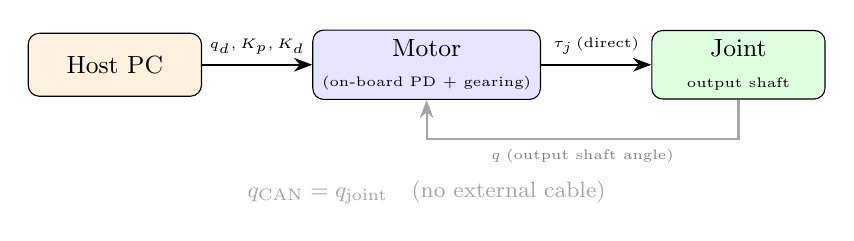
\begin{tikzpicture}[>=Stealth, node distance=1.3cm, every node/.style={font=\small, align=center}]
  % nodes
  \node[draw, rounded corners, fill=orange!12, minimum width=2.2cm, minimum height=0.8cm]
      (host) {Host PC};
  \node[draw, rounded corners, fill=blue!10, minimum width=2.6cm, minimum height=0.8cm,
        right=1.4cm of host] (motor) {Motor\\\tiny(on-board PD + gearing)};
  \node[draw, rounded corners, fill=green!12, minimum width=2.2cm, minimum height=0.8cm,
        right=1.4cm of motor] (joint) {Joint\\\tiny output shaft};
  % arrows forward
  \draw[->, thick] (host) -- node[above,font=\tiny]{$q_d, K_p, K_d$} (motor);
  \draw[->, thick] (motor) -- node[above,font=\tiny]{$\tau_j$\,(direct)} (joint);
  % feedback arrow (bottom)
  \draw[->, thick, gray!70] (joint.south) -- ++(0,-0.5) -|
      node[below, pos=0.25, font=\tiny, gray]{$q$\;(output shaft angle)} (motor.south);
  % note
  \node[font=\footnotesize, below=0.9cm of motor, text=gray!70]
      {$q_{\mathrm{CAN}} = q_{\mathrm{joint}}$\quad (no external cable)};
\end{tikzpicture}
\caption{Traditional servo robot (and our \textbf{shoulder}): motor sends torque directly
to the joint.  CAN feedback angle equals joint angle.  No spring, no cable lag.}
\label{fig:traditional}
\end{figure}

\begin{resultbox}
In a rigid-transmission robot, $q_{\mathrm{motor}}\!=\!q_{\mathrm{joint}}$ always.
The PD loop closes on the actual joint position.  No spring, no lag, no compliance.
High $K_p$ is safe.
\end{resultbox}

% -------------------------------------------------------------------------
\subsection{Our Arm: Two Motors, Two Joints, One Encoder}
\label{sec:ourarm_overview}
% -------------------------------------------------------------------------

Our arm differs from the traditional case in two ways:

\begin{enumerate}[leftmargin=2em]
  \item \textbf{Shoulder ($q_1$)} behaves like a traditional direct-drive joint.
        Motor shaft connects rigidly to Link~1; $q_1 = \theta_{m1}$ (CAN reports output shaft angle directly).
  \item \textbf{Elbow ($q_2$)} is driven through a \textbf{direct steel cable}
        (no spring in the drive cable path, current setup).  Once the cable
        is wound taut, motor angle $\approx$ joint angle.  The AS5048A
        absolute encoder reads the true joint angle directly from the joint
        axis and is the primary feedback source.
\end{enumerate}

The \textbf{exo cable} (Damiao motor) \emph{does} have a spring inserted
via key rings (see Case~B).d taut, motor angle $\approx$ joint angle.  The AS5048A
        absolute encoder reads the true joint angle directly from the joint
        axis and is the primary feedback source.
\end{enumerate}

The \textbf{exo cable} (Damiao motor) \emph{does} have a spring inserted
via key rings (see Case~B).

\begin{figure}[H]
\centering
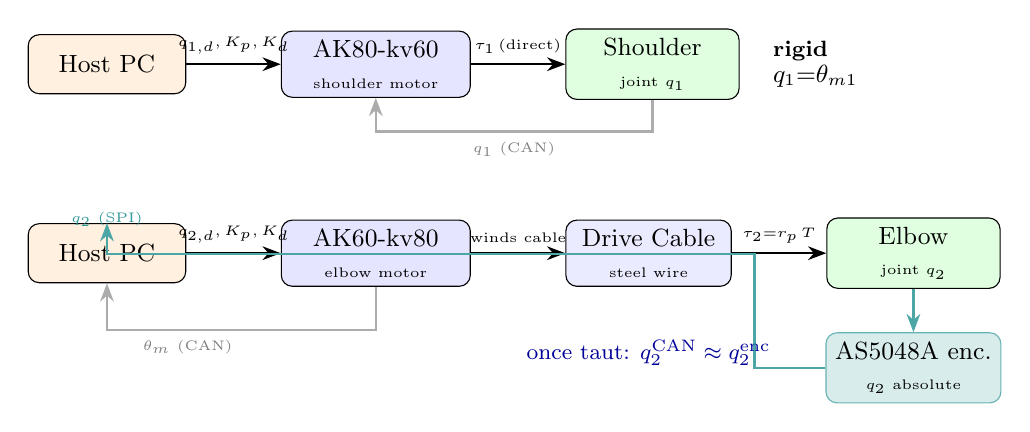
\begin{tikzpicture}[>=Stealth, node distance=0.0cm, every node/.style={font=\small, align=center}]

  %% ─── Shoulder row ───────────────────────────────────────────────────────
  \node[draw, rounded corners, fill=orange!12,
        minimum width=2.0cm, minimum height=0.75cm] (sh_host)
      at (0, 0) {Host PC};

  \node[draw, rounded corners, fill=blue!10,
        minimum width=2.4cm, minimum height=0.75cm,
        right=1.2cm of sh_host] (sh_motor)
      {AK80-kv60\\\tiny shoulder motor};

  \node[draw, rounded corners, fill=green!12,
        minimum width=2.2cm, minimum height=0.75cm,
        right=1.2cm of sh_motor] (sh_joint)
      {Shoulder\\\tiny joint $q_1$};

  \draw[->, thick] (sh_host) -- node[above,font=\tiny]{$q_{1,d},K_p,K_d$} (sh_motor);
  \draw[->, thick] (sh_motor) -- node[above,font=\tiny]{$\tau_1$\,(direct)} (sh_joint);
  \draw[->, thick, gray!65] (sh_joint.south) -- ++(0,-0.4) -|
      node[below,pos=0.25,font=\tiny,gray]{$q_1$ (CAN)} (sh_motor.south);

  \node[right=0.3cm of sh_joint, font=\footnotesize, align=left]
      {\textbf{rigid}\\\small $q_1{=}\theta_{m1}$};

  %% ─── Elbow row ──────────────────────────────────────────────────────────
  \node[draw, rounded corners, fill=orange!12,
        minimum width=2.0cm, minimum height=0.75cm] (el_host)
      at (0, -2.4) {Host PC};

  \node[draw, rounded corners, fill=blue!10,
        minimum width=2.4cm, minimum height=0.75cm,
        right=1.2cm of el_host] (el_motor)
      {AK60-kv80\\\tiny elbow motor};

  \node[draw, rounded corners, fill=blue!8,
        minimum width=2.1cm, minimum height=0.75cm,
        right=1.2cm of el_motor] (cable)
      {Drive Cable\\\tiny steel wire};

  \node[draw, rounded corners, fill=green!12,
        minimum width=2.2cm, minimum height=0.75cm,
        right=1.2cm of cable] (el_joint)
      {Elbow\\\tiny joint $q_2$};

  \node[draw, rounded corners, fill=teal!15, draw=teal!60,
        minimum width=2.2cm, minimum height=0.75cm,
        below=0.55cm of el_joint] (enc)
      {AS5048A enc.\\\tiny $q_2$ absolute};

  \draw[->, thick] (el_host) -- node[above,font=\tiny]{$q_{2,d},K_p,K_d$} (el_motor);
  \draw[->, thick] (el_motor) -- node[above,font=\tiny]{winds cable} (cable);
  \draw[->, thick] (cable) -- node[above,font=\tiny]{$\tau_2{=}r_p\,T$} (el_joint);
  %% encoder reads joint
  \draw[->, thick, teal!70] (el_joint.south) -- (enc.north);
  %% CAN feedback to motor (motor-side only)
    \draw[->, thick, gray!65] (el_motor.south) -- ++(0,-0.55) -|
      node[below,pos=0.35,font=\tiny,gray]{$\theta_m$ (CAN)} (el_host.south);
  %% encoder to host
    \draw[->, thick, teal!70] (enc.west) -- ++(-0.9,0) -- ++(0,1.45) -|
      node[above,pos=0.78,font=\tiny,teal!80]{$q_2$ (SPI)} (el_host.north);

  %% annotation: taut cable -> q_CAN ≈ q_enc
    \node[font=\footnotesize, below=0.55cm of cable, blue!60!black]
      {once taut: $q_2^{\mathrm{CAN}} \approx q_2^{\mathrm{enc}}$};

\end{tikzpicture}
\caption{Our arm signal flow.
  \textbf{Shoulder}: rigid direct drive ($q_1 = \theta_{m1}$).
  \textbf{Elbow}: direct steel cable (no spring); once taut, CAN angle
  $\approx$ encoder angle.  The AS5048A reads the true joint angle via SPI
  and is the primary elbow feedback source.}
\label{fig:ourarm_flow}
\end{figure}

% -------------------------------------------------------------------------
\subsection{Case A: Drive Cable (No Spring) --- Manual Home Positioning}
\label{sec:caseA}
% -------------------------------------------------------------------------

\textbf{This is the current hardware configuration for the elbow drive cable.}
The steel cable runs from the motor drum, over the 623zz idler bearings, and
directly onto the elbow joint drum --- no spring in the cable path.

\textbf{Key advantage:} any joint angle can be set as the home position
\emph{on every startup}.  You simply hold the arm at your desired angle,
set the encoder zero, and enable low-tension mode.  This is flexible and safe.

\paragraph{Why this works for any control scheme.}
When you call \texttt{set\_zero(burn\_otp=False)}, you are \textbf{redefining the reference frame}
for angle measurements. All control laws (CT, LQR, impedance) depend only on
\emph{relative} angles and velocities, not on an absolute world reference.

\begin{itemize}[leftmargin=2em]
  \item \textbf{Gravity term} $g(q)$: Depends only on angle $q$ relative to home.
        If you hold at any position and set zero there, gravity is correctly
        computed relative to that custom reference frame.
  \item \textbf{Inertia} $M(q)$ and \textbf{Coriolis} $C(q,\dot{q})$: Purely kinematic;
        invariant to reference frame shifts.
  \item \textbf{Feedback error} $(q_d - q)$: Still valid; error is measured in your
        coordinate system.
\end{itemize}

Therefore, \textbf{flexible any-angle home is compatible with CT, LQR, and all
other control laws}. It is purely a change of reference frame, not a change in dynamics.

% ------------------------------------------------------------------
\paragraph{Alternative home-positioning methods.}
% ------------------------------------------------------------------
There are three practical ways to set a home position.
Table~\ref{tab:home_methods} compares them, including which methods
\textbf{require manual holding} and which are fully automated.

\begin{table}[H]
\centering
\small
\begin{tabular}{p{3.0cm} p{3.2cm} p{3.4cm} p{1.4cm} p{1.2cm}}
\toprule
\textbf{Method} & \textbf{How} & \textbf{Pros / Cons} & \textbf{Persists?} & \textbf{Hold?} \\
\midrule

\textbf{A. Manual hold +\newline RAM zero} \newline
\emph{(used in this section)}
&
Hold arm at desired angle, call \texttt{set\_zero(burn\_otp=False)}
&
\textcolor{green!60!black}{+ Any angle as home, fully flexible}\newline
\textcolor{green!60!black}{+ Safe: low-tension from home}\newline
\textcolor{orange!80!black}{-- Must redo every power-on}
&
RAM only\newline(lost on\newline power-off)
&
\textcolor{orange!80!black}{Yes (each\newline startup)} \\

\midrule

\textbf{B. OTP burn}\newline
\emph{(optional, documented below)}
&
Same as A, then call \texttt{set\_zero(burn\_otp=True)} once
&
\textcolor{green!60!black}{+ Auto-zero every power-on}\newline
\textcolor{green!60!black}{+ \textbf{No hold needed after burn}}\newline
\textcolor{red!70!black}{-- One-time only, irreversible}
&
Permanent\newline(OTP fuse)
&
\textcolor{orange!80!black}{Once only} \\

\midrule

\textbf{C. Software offset}\newline
\emph{(no hardware write)}
&
Read raw encoder, subtract a constant:\newline
\texttt{q = enc.read() - HOME\_OFFSET}
&
\textcolor{green!60!black}{+ No encoder modification}\newline
\textcolor{green!60!black}{+ Easily changeable in code}\newline
\textcolor{orange!80!black}{-- Must store offset externally}
&
In code /\newline config file
&
\textcolor{orange!80!black}{Yes (each\newline startup)} \\

\bottomrule
\end{tabular}
\caption{Comparison of home-positioning methods for the elbow joint.}
\label{tab:home_methods}
\end{table}

\begin{tcolorbox}[colback=green!5, colframe=green!50!black, title=\textbf{Recommended method}]
  \textbf{To skip manual holding altogether:}
  \begin{itemize}[leftmargin=1.5em]
    \item \textbf{Method B (OTP burn)}: Hold the arm \emph{once today}, burn the zero.
          Every future startup is fully automatic --- no holding ever again.
          This is the best long-term solution.
  \end{itemize}
  \textbf{Method A (manual hold + RAM zero)} is recommended during development:
  flexible, safe, no hardware commitment. Once home is confirmed, promote to Method B.
\end{tcolorbox}

\medskip

\textbf{Method C: software offset (code example).}
If you prefer not to call \texttt{set\_zero()} at all, just store the raw angle at startup
and subtract it throughout the session:
\begin{lstlisting}[caption={Software offset: no encoder write needed.}]
with AS5048A(AS5048AConfig()) as enc:
    # Record raw angle at current position (= your chosen home)
    HOME_OFFSET = enc.read_angle_rad()

# ... later in control loop:
q2 = enc.read_angle_rad() - HOME_OFFSET   # relative to home
\end{lstlisting}

\paragraph{Step-by-step procedure (Method A).}

\begin{tcolorbox}[colback=gray!5, colframe=gray!50, title=\textbf{Two joints --- two different home strategies}]
\begin{tabularx}{\linewidth}{@{}lXX@{}}
\toprule
\textbf{Joint} & \textbf{Sensor} & \textbf{Home method} \\
\midrule
Shoulder $q_1$ & CAN only (no encoder) &
  \textbf{OTP burn once}; offset persists across power cycles \\
Elbow $q_2$ & CAN + AS5048A encoder &
  \textbf{RAM zero each session}; AS5048A gives independent angle \\
\bottomrule
\end{tabularx}

\smallskip
The procedure below covers \textbf{both joints in parallel}.
Shoulder notes: \textcolor{blue!70!black}{\textbf{[SHOULDER]}};
elbow notes: \textcolor{green!50!black}{\textbf{[ELBOW]}}.
\end{tcolorbox}

\begin{figure}[H]
\centering
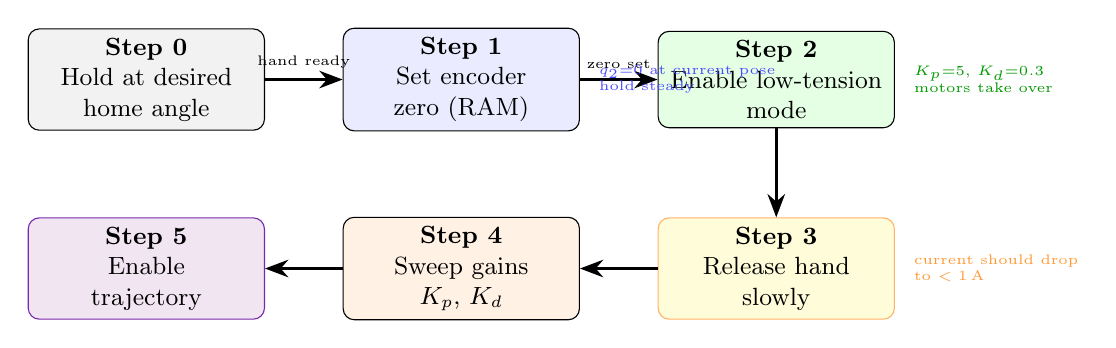
\begin{tikzpicture}[>=Stealth, every node/.style={font=\small, align=center}]
  \def\bw{3.0cm}  \def\bh{1.0cm}

  \node[draw, rounded corners=4pt, fill=gray!10,
        minimum width=\bw, minimum height=\bh] (s0)
      at (0,0) {\textbf{Step 0}\\Hold at desired\\home angle};

  \node[draw, rounded corners=4pt, fill=blue!8,
        minimum width=\bw, minimum height=\bh] (s1)
      at ($(s0)+(4.0,0)$) {\textbf{Step 1}\\Set encoder\\zero (RAM)};

  \node[draw, rounded corners=4pt, fill=green!10,
        minimum width=\bw, minimum height=\bh] (s2)
      at ($(s1)+(4.0,0)$) {\textbf{Step 2}\\Enable low-tension\\mode};

  \node[draw, rounded corners=4pt, fill=yellow!15, draw=orange!60,
        minimum width=\bw, minimum height=\bh] (s3)
      at ($(s2)+(0,-2.4)$) {\textbf{Step 3}\\Release hand\\slowly};

  \node[draw, rounded corners=4pt, fill=orange!10,
        minimum width=\bw, minimum height=\bh] (s4)
      at ($(s1)+(0,-2.4)$) {\textbf{Step 4}\\Sweep gains\\$K_p$, $K_d$};

  \node[draw, rounded corners=4pt, fill=violet!10, draw=exopurple,
        minimum width=\bw, minimum height=\bh] (s5)
      at ($(s0)+(0,-2.4)$) {\textbf{Step 5}\\Enable\\trajectory};

  \draw[->, very thick] (s0) -- node[above,font=\tiny]{hand ready} (s1);
  \draw[->, very thick] (s1) -- node[above,font=\tiny]{zero set} (s2);
  \draw[->, very thick] (s2) -- (s3);
  \draw[->, very thick] (s3) -- (s4);
  \draw[->, very thick] (s4) -- (s5);

  \node[font=\tiny, align=left, right=0.12cm of s1, text=blue!70]
      {$q_2{=}0$ at current pose\\hold steady};
  \node[font=\tiny, align=left, right=0.12cm of s2, text=green!60!black]
      {$K_p{=}5$, $K_d{=}0.3$\\motors take over};
  \node[font=\tiny, align=left, right=0.12cm of s3, text=orange!80]
      {current should drop\\to $<1$\,A};
\end{tikzpicture}
\caption{Commissioning flow: hold arm at any desired home angle, then low-tension takeover.}
\label{fig:commissioning_flow_A}
\end{figure}

\paragraph{Step 0 --- Hold arm at desired home angle.}
Place the arm at \textbf{any angle you want to be ``home''} (fully extended, elbow
at 90°, flexed, etc.).  Support the weight with your hand and keep it steady.
The cable will be slack initially --- motors are off.

\textbf{Example.}
Suppose you want startup home to be: shoulder pointing 30° forward from the base,
and elbow bent at 90°.  Manually hold the arm in exactly that pose.
Nothing is ``zero'' yet --- you are only choosing the physical pose that will later
be called $(q_1,q_2) = (0,0)$.
\begin{lstlisting}[caption={Hand-position the arm at desired home.}]
input("1. Position arm at DESIRED HOME ANGLE.\n"
      "   Support weight with your hand.\n"
      "   Press Enter when ready...")
\end{lstlisting}

\paragraph{Step 1 --- Set encoder zero at current position.}
Read the encoder and set it to zero \textbf{in RAM} (not permanent OTP).
This makes the current position ``$q_2 = 0$'' for this session.

\textcolor{blue!70!black}{\textbf{[SHOULDER]}}: No AS5048A --- use the CAN motor angle directly.
The motor reports its current output shaft angle; record this as the shoulder home reference.
For repeatable startup, burn OTP once (see end of this section).

\textcolor{green!50!black}{\textbf{[ELBOW]}}: Use the AS5048A absolute encoder.
This gives the true joint angle, independent of cable spring deflection.

\textbf{Example.}
At the held pose from Step~0, the shoulder CAN may read $q_1 = 27.4°$ and the elbow
AS5048A may read $q_2 = 91.2°$.  After this step, the controller will treat those same
physical angles as the home reference: shoulder target stored as \texttt{q1\_start = 27.4°},
and elbow encoder reset so it now reports approximately $0.0°$ at that same pose.

\begin{lstlisting}[caption={Set zeros for both joints.}]
# --- SHOULDER: CAN-only zero (no secondary encoder) ---
q1_start, _, _ = shoulder.read_state()["shoulder"]
print(f"Shoulder CAN zero: {np.rad2deg(q1_start):.1f}deg")
# q1_start is the motor output-shaft angle at home;
# controller uses relative error (q_d - q1_start)
# Recommend burning this to OTP once confirmed (see end of section)

# --- ELBOW: AS5048A absolute encoder zero ---
with AS5048A(AS5048AConfig()) as enc:
    enc.set_zero(burn_otp=False)    # RAM only, temporary
    q2_zero = enc.read_angle_rad()
    print(f"Elbow encoder zero set. Current angle: {np.rad2deg(q2_zero):.1f}deg")
\end{lstlisting}

\paragraph{Step 2 --- Enable low-tension mode.}
Power on both motors with \textbf{very low} $K_p$ (5).  The motors will start holding
the arm at the position you're still supporting with your hand.
The cable begins to wind up but with minimal force.

\textbf{Example.}
If you are still holding the chosen home pose, commanding
\texttt{shoulder = q1\_start} and \texttt{elbow = 0.0} with low gains means the motors
take over gently.  You should feel only a light holding force, not a sharp pull.
\begin{lstlisting}[caption={Motors take over with low tension.}]
print("2. Motors powering on (low tension)...")
shoulder.write("goal_position", {"shoulder": q1_start}, kp=5.0, kd=0.3)
elbow.write(   "goal_position", {"elbow":    0.0},  kp=5.0, kd=0.3)  # 0 = home
time.sleep(0.3)
\end{lstlisting}

\paragraph{Step 3 --- Slowly release your hand.}
Gradually let go over 1--2 seconds.  Watch the motor current on the console.
As you release, motor current should \textbf{drop toward zero} (cable slack remaining,
both cables neutral).  If current rises steeply, you may not be at a true zero position
--- arm is not at mechanical equilibrium.

\textbf{Example.}
Good release case: shoulder current settles near $0.2$--$0.4$\,A and elbow current settles
near $0.3$\,A, with the arm staying in place.
Bad release case: elbow current rises to $2.5$\,A and the joint creeps a few degrees,
which means the elbow zero was set away from the neutral cable position --- redo from Step~0.

\begin{warnbox}
  \textbf{Check motor current during release --- both joints.}
  
  \begin{itemize}[leftmargin=2em]
    \item \textcolor{blue!70!black}{\textbf{[SHOULDER]}} --- direct-drive, no cable spring:
      current should drop to near $0$\,A immediately on release.
      A steady current $>1$\,A means the shoulder home angle was set while
      the motor shaft was not at its cable equilibrium.
    \item \textcolor{green!50!black}{\textbf{[ELBOW]}} --- antagonistic cable SEA:\newline
      Current $< 0.5$\,A after release: ✓ both cables neutral.\newline
      Current $1$--$2$\,A: ⚠ arm is off the neutral cable position; acceptable but not ideal.\newline
      Current $> 2$\,A: ✗ wrong zero angle --- redo from Step~0.
  \end{itemize}
\end{warnbox}

\begin{lstlisting}[caption={Monitor current while releasing.}]
print("3. Release your hand slowly. Watch current below:")
for i in range(10):
    _, _, i_a = elbow.read_state()["elbow"]
    q2_enc    = enc.read_angle_rad()
    print(f"   Current: {i_a:.2f} A  |  Encoder: {np.rad2deg(q2_enc):.1f}°")
    time.sleep(0.3)
\end{lstlisting}

\paragraph{Step 4 --- Sweep gains.}
Once the arm is stable on the motors, increase $K_p$ gradually in steps to reach
operating gains.  Monitor for oscillation.
Target range: $K_p = 30$--$50$, $K_d = 0.8$--$1.5$.

\textbf{Example.}
You might test $K_p = 5, 10, 20, 30, 40$ while keeping the arm at home.
If the arm stays quiet up to $K_p = 30$ but starts buzzing or overshooting at $K_p = 40$,
then $K_p = 30$ with slightly larger $K_d$ is a safer operating choice.
\begin{lstlisting}[caption={Ramp up gains from 5 to 40.}]
for kp in [5, 10, 15, 20, 30, 40]:
    shoulder.write("goal_position", {"shoulder": q1_start}, kp=kp, kd=0.5)
    elbow.write(   "goal_position", {"elbow":    0.0},     kp=kp, kd=0.5)
    print(f"Testing Kp={kp}...")
    time.sleep(1.0)
print("✓ Gains stable. Ready for trajectory.")
\end{lstlisting}

\paragraph{Step 5 --- Enable trajectory.}
Send your first trajectory command.  The encoder zero you set remains valid for the
entire session.

\textbf{Example.}
If the chosen home pose is the arm's comfortable resting pose, then a command like
$q_1^d = q_{1,\mathrm{start}} + 0.3\sin(0.3t)$ and $q_2^d = 0.0 + 0.2\sin(0.5t)$
means the shoulder oscillates around its stored startup angle, while the elbow oscillates
around the newly defined home angle $q_2 = 0$.
\begin{lstlisting}[caption={Send trajectory (example: sine wave).}]
t0 = time.monotonic()
while True:
    t  = time.monotonic() - t0
    # Oscillate around the home position
    q1_d = q1_start + 0.3 * np.sin(0.3*t)
    q2_d =      0.0 + 0.2 * np.sin(0.5*t)  # 0 is home
    
    shoulder.write("goal_position", {"shoulder": q1_d}, kp=40.0, kd=1.2)
    elbow.write(   "goal_position", {"elbow":    q2_d}, kp=30.0, kd=1.0)
    time.sleep(0.01)
\end{lstlisting}

\paragraph{Optional: Burn elbow encoder zero to OTP (permanent).}
If you want the \textbf{elbow} home to survive power cycles, burn the AS5048A zero permanently
after you've verified the arm is stable:

\begin{lstlisting}[caption={Permanently burn elbow OTP zero (one-time only).}]
print("Burning ELBOW encoder zero to OTP (PERMANENT, IRREVERSIBLE)...")
with AS5048A(AS5048AConfig()) as enc:
    enc.set_zero(burn_otp=True)
print("OTP burned. This angle will be zero on every future power-up.")
\end{lstlisting}

\paragraph{Shoulder: burn CAN zero to OTP (recommended once).}
The shoulder has \textbf{no secondary encoder} --- it relies entirely on the CAN motor angle.
Because the CAN zero is lost on power-off unless burned, burn OTP once
after confirming the mechanical home.

\textbf{When to burn:} after Step~3 confirms low current (stable home), and before
running any trajectory.

\begin{lstlisting}[caption={Burn shoulder home to OTP --- run once only.}]
# SHOULDER: burn current CAN angle as permanent zero
# ONLY run this after Step 3 confirms low current (correct home)
print("Burning SHOULDER zero to OTP (PERMANENT, IRREVERSIBLE)...")
shoulder.encoder.set_zero(burn_otp=True)
# Verify: CAN should now report ~0.0 deg
q1_check, _, _ = shoulder.read_state()["shoulder"]
print(f"Shoulder CAN after burn: {np.rad2deg(q1_check):.1f}deg  (expect ~0.0)")
print("Done. Shoulder home will load automatically on every future power-on.")
\end{lstlisting}

\begin{tcolorbox}[colback=orange!5, colframe=orange!60, title=\textbf{Shoulder vs Elbow: OTP lifetime rule}]
\begin{itemize}[leftmargin=1.5em]
  \item \textcolor{blue!70!black}{\textbf{Shoulder}}: OTP burn is \textbf{essential} for reproducibility
        (no absolute encoder to re-zero each session).  Burn once when home is confirmed.
  \item \textcolor{green!50!black}{\textbf{Elbow}}: OTP burn is \textbf{optional}.
        The AS5048A lets you re-zero in RAM every session with no loss of accuracy.
        Only burn OTP once your home angle is finalized.
  \item \textbf{Both}: OTP fuses are one-time only.  Use \texttt{burn\_otp=False} during development.
\end{itemize}
\end{tcolorbox}

\paragraph{How burning works.}
When you call \texttt{set\_zero(burn\_otp=True)}, the AS5048A records the \textbf{current magnetic angle to permanent fuses}.
The magnet is bolted to the joint --- it is purely passive (no power needed).

On every future power-on:
\begin{enumerate}[leftmargin=2em]
  \item The sensor wakes up and reads the magnet position (always accurate).
  \item It subtracts the burned OTP offset automatically.
  \item Output $= \text{(current magnet angle)} - \text{(burned OTP offset)}$.
\end{enumerate}

\paragraph{Safe to move the joint while powered off.}
The magnet is the source of truth --- it does \textbf{not} require power.
If you manually rotate the joint while the sensor is off:
\begin{itemize}[leftmargin=2em]
  \item The magnet rotates with the joint (mechanically coupled).
  \item When you power on, the sensor reads the magnet's \textbf{new position}.
  \item Output is still correct because it's always relative to the burned offset.
\end{itemize}

\textbf{Example:} If OTP burned at 0° and you manually move the joint to 60° while powered off,
the sensor powers on and reads: $60° - 0° = 60°$ ✓

\begin{warnbox}
  \textbf{Each encoder can only burn OTP \textbf{once} --- this is irreversible.}
  Only use `burn\_otp=True` when you are certain of your home position.
  For experimentation, use `burn\_otp=False` (RAM only, cleared on power-off).
  
  \textbf{Safe to physically move the arm when powered off.}
  The magnet is passive --- no homing sequence needed after power-on.
\end{warnbox}

% -------------------------------------------------------------------------
% -------------------------------------------------------------------------
\subsection{Case B: Exo Cable (Spring via Key Rings) --- Damiao Motor}
\label{sec:caseB}
% -------------------------------------------------------------------------

\textbf{This applies to the exo cable only.}
The Damiao motor drives a steel cable that has a \textbf{coil spring inserted
mid-span via two key rings} (quick-links):
\[
  \underbrace{\text{Damiao drum}\;\to\;\text{routing}\;\to\;\text{cable}}_{\text{upper half}}
  \;\xrightarrow{\text{key ring}}\;
  \underbrace{\text{spring}\;(k_{\mathrm{exo}})}_{\text{elastic element}}
  \;\xrightarrow{\text{key ring}}\;
  \underbrace{\text{cable}\;\to\;\text{elbow joint drum}}_{\text{lower half}}
\]
The spring makes the exo cable compliant: torque is proportional to deflection
$\delta_e = r_{\mathrm{exo}}(\theta_{me} - q_2)$.
The bring-up is more involved because:
\begin{itemize}[leftmargin=2em]
  \item The cable may be \textbf{slack} at power-on.
  \item Damiao CAN angle $\theta_{me} \neq q_2$ (spring deflection unknown at power-on).
  \item A stiff command before the cable is taut can snap or tangle it.
\end{itemize}

\paragraph{Step-by-step procedure.}

\begin{figure}[H]
\centering
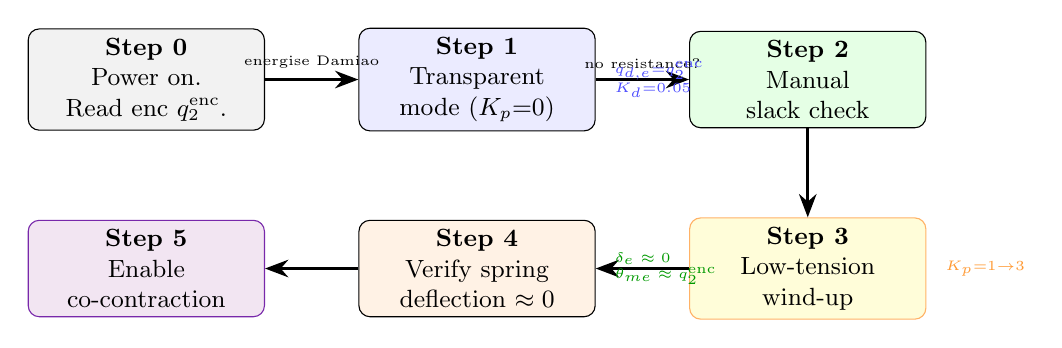
\begin{tikzpicture}[>=Stealth, every node/.style={font=\small, align=center}]
  \def\bw{3.0cm}  \def\bh{1.0cm}

  \node[draw, rounded corners=4pt, fill=gray!10,
        minimum width=\bw, minimum height=\bh] (s0)
      at (0,0) {\textbf{Step 0}\\Power on.\\Read enc $q_2^{\mathrm{enc}}$.};

  \node[draw, rounded corners=4pt, fill=blue!8,
        minimum width=\bw, minimum height=\bh] (s1)
      at ($(s0)+(4.2,0)$) {\textbf{Step 1}\\Transparent\\mode ($K_p{=}0$)};

  \node[draw, rounded corners=4pt, fill=green!10,
        minimum width=\bw, minimum height=\bh] (s2)
      at ($(s1)+(4.2,0)$) {\textbf{Step 2}\\Manual\\slack check};

  \node[draw, rounded corners=4pt, fill=yellow!15, draw=orange!60,
        minimum width=\bw, minimum height=\bh] (s3)
      at ($(s2)+(0,-2.4)$) {\textbf{Step 3}\\Low-tension\\wind-up};

  \node[draw, rounded corners=4pt, fill=orange!10,
        minimum width=\bw, minimum height=\bh] (s4)
      at ($(s1)+(0,-2.4)$) {\textbf{Step 4}\\Verify spring\\deflection $\approx 0$};

  \node[draw, rounded corners=4pt, fill=violet!10, draw=exopurple,
        minimum width=\bw, minimum height=\bh] (s5)
      at ($(s0)+(0,-2.4)$) {\textbf{Step 5}\\Enable\\co-contraction};

  \draw[->, very thick] (s0) -- node[above,font=\tiny]{energise Damiao} (s1);
  \draw[->, very thick] (s1) -- node[above,font=\tiny]{no resistance?} (s2);
  \draw[->, very thick] (s2) -- (s3);
  \draw[->, very thick] (s3) -- (s4);
  \draw[->, very thick] (s4) -- (s5);

  \node[font=\tiny, align=left, right=0.12cm of s1, text=blue!70]
      {$q_{d,e}{=}q_2^{\mathrm{enc}}$\\$K_d{=}0.05$};
  \node[font=\tiny, align=left, right=0.12cm of s3, text=orange!80]
      {$K_p{=}1{\to}3$};
  \node[font=\tiny, align=left, right=0.12cm of s4, text=green!60!black]
      {$\delta_e \approx 0$\\$\theta_{me} \approx q_2^{\mathrm{enc}}$};
\end{tikzpicture}
\caption{Commissioning flow for the exo cable (Damiao, spring via key rings).}
\label{fig:commissioning_flow_B}
\end{figure}

\paragraph{Step 0 --- Power on, read elbow encoder.}
Read the elbow angle before energising the Damiao.  This angle will be the
transparent-mode target.\
\begin{lstlisting}[caption={Read elbow angle before energising Damiao.}]
q2_enc = enc.read_angle_rad()   # absolute, no homing
print(f"Elbow at power-on: {np.rad2deg(q2_enc):.1f} deg")
\end{lstlisting}

\paragraph{Step 1 --- Set Damiao to transparent mode.}
$K_p = 0$, light damping only.  The motor tracks $q_2^{\mathrm{enc}}$ so
cable extension is zero: $\delta_e \approx 0$, no force on the joint.
\begin{lstlisting}[caption={Damiao transparent mode from power-on.}]
exo.write("mit_command", {"exo": q2_enc},
          kp=0.0, kd=0.05, tau_ff=0.0)   # zero tension
\end{lstlisting}

\paragraph{Step 2 --- Manual slack check.}
With the Damiao in transparent mode, \textbf{manually flex the elbow slowly}.
The exo cable should offer \emph{no resistance}.  If you feel tension,
check the key-ring attachment direction.

\begin{warnbox}
  \textbf{Check key-ring and spring orientation.}
  The spring must extend when the cable is pulled (not compressed).
  A reversed connection means the spring is buckled rather than stretched ---
  the cable will feel stiff in the wrong direction and may tangle.
\end{warnbox}

\paragraph{Step 3 --- Low-tension wind-up.}
Slowly increase $K_p$ to gently take up any cable slack, still targeting
$q_{d,e} = q_2^{\mathrm{enc}}$.
\begin{lstlisting}[caption={Low-tension wind-up for exo cable.}]
for kp in [1.0, 2.0, 3.0]:          # ramp Kp in steps
    exo.write("mit_command", {"exo": enc.read_angle_rad()},
              kp=kp, kd=0.3, tau_ff=0.0)
    time.sleep(0.3)
\end{lstlisting}

\paragraph{Step 4 --- Verify spring deflection near zero.}
At rest the Damiao CAN angle should satisfy $\theta_{me} \approx q_2^{\mathrm{enc}}$.
Their difference equals the spring deflection $\delta_e / r_{\mathrm{exo}}$.
\begin{lstlisting}[caption={Check spring deflection at rest.}]
theta_me, _, _ = exo.read_state()["exo"]
q2_enc         = enc.read_angle_rad()
delta_e = 0.04775 * (theta_me - q2_enc)     # deflection [m]
print(f"Spring deflection: {delta_e*1000:.1f} mm  (expect ~0 at rest)")
\end{lstlisting}

\paragraph{Step 5 --- Enable co-contraction.}
Activate with a small offset $\Delta\theta$ to pre-tension the spring.
\begin{lstlisting}[caption={Enable exo co-contraction.}]
DELTA_THETA = np.deg2rad(5.0)   # 5 deg -> gentle pre-tension
exo.write("mit_command",
          {"exo": enc.read_angle_rad() + DELTA_THETA},
          kp=5.0, kd=0.3, tau_ff=0.0)
\end{lstlisting}

\begin{warnbox}
  \textbf{Never activate co-contraction before completing Steps~1--4.}
  A large $\Delta\theta$ with stiff gains on a slack cable will snap the
  spring-cable assembly onto the elbow joint drum, jerking the elbow joint.
\end{warnbox}

% -------------------------------------------------------------------------
\subsection{Why Cable Compliance Changes Everything vs.\ Traditional Control}
\label{sec:compare}
% -------------------------------------------------------------------------

\begin{figure}[H]
\centering
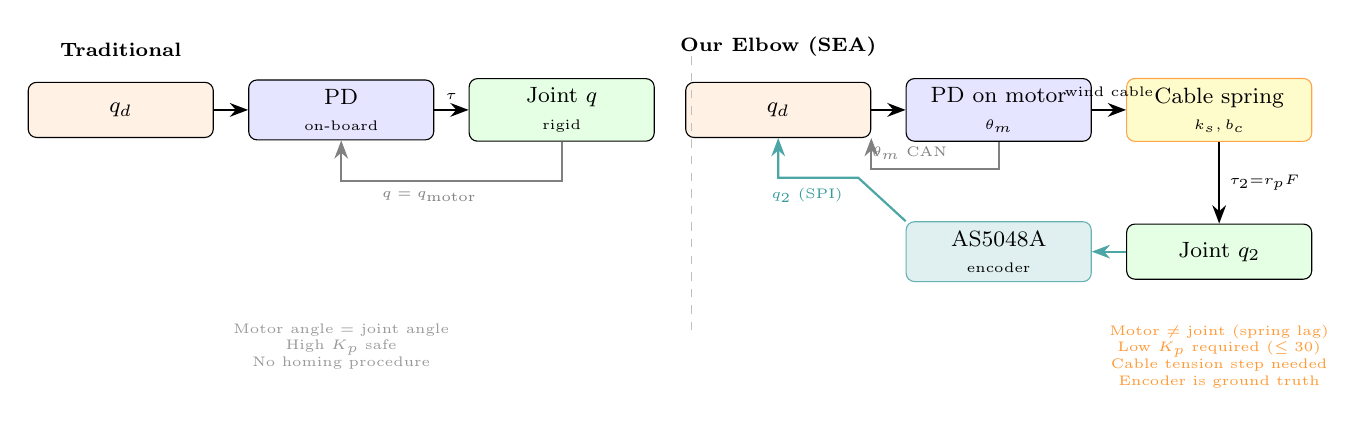
\begin{tikzpicture}[>=Stealth, every node/.style={font=\footnotesize},
  box/.style={draw, rounded corners=3pt, minimum width=2.35cm,
              minimum height=0.7cm, align=center}]

  %% ─── Left: traditional ─────────────────────────────────────────────────
  \node[box, fill=orange!10]       (td_ref)   at (0, 0)    {$q_d$};
  \node[box, fill=blue!10]         (td_pid)   at (2.8, 0)  {PD\\\tiny on-board};
  \node[box, fill=green!10]        (td_joint) at (5.6, 0)  {Joint $q$\\\tiny rigid};
  \draw[->, thick] (td_ref) -- node[above,font=\tiny]{} (td_pid);
  \draw[->, thick] (td_pid) -- node[above,font=\tiny]{$\tau$} (td_joint);
  \draw[->, thick, gray] (td_joint.south) -- ++(0,-0.5) -|
      node[below,font=\tiny,gray,pos=0.3]{$q = q_{\mathrm{motor}}$} (td_pid.south);
  \node[font=\scriptsize\bfseries, above=0.2cm of td_ref] {Traditional};

  %% ─── Right: our SEA elbow ───────────────────────────────────────────────
    \node[box, fill=orange!10]       (se_ref)   at (8.35, 0)    {$q_d$};
    \node[box, fill=blue!10]         (se_pid)   at (11.15, 0)   {PD on motor\\\tiny $\theta_m$};
    \node[box, fill=yellow!20, draw=orange!70] (se_spring) at (13.95, 0)
      {Cable spring\\\tiny $k_s, b_c$};
    \node[box, fill=green!10]        (se_joint) at (13.95,-1.8) {Joint $q_2$};
    \node[box, fill=teal!12, draw=teal!60] (se_enc) at (11.15,-1.8)
      {AS5048A\\\tiny encoder};

  \draw[->, thick] (se_ref) -- (se_pid);
    \draw[->, thick] (se_pid) -- node[above,font=\tiny,yshift=1pt]{wind cable} (se_spring);
  \draw[->, thick] (se_spring) -- node[right,font=\tiny]{$\tau_2{=}r_pF$} (se_joint);
  \draw[->, thick, teal!70] (se_joint) -- (se_enc);
    \draw[->, thick, teal!70] (se_enc.north west) -- ++(-0.6,0.55) -|
      node[below,font=\tiny,teal!80,pos=0.32]{$q_2$ (SPI)} (se_ref.south);
    \draw[->, thick, gray] (se_pid.south) -- ++(0,-0.35) -|
      node[above,font=\tiny,gray,pos=0.35]{$\theta_m$ CAN} (se_ref.south east);
  \node[font=\scriptsize\bfseries, above=0.2cm of se_ref] {Our Elbow (SEA)};

  %% ─── Comparison notes ──────────────────────────────────────────────────
    \draw[dashed, gray!50] (7.25, -2.8) -- (7.25, 0.8);
  \node[font=\tiny, align=center, below=2.2cm of td_pid, text=gray!80]
      {Motor angle = joint angle\\High $K_p$ safe\\No homing procedure\\};
  \node[font=\tiny, align=center, below=2.2cm of se_spring, text=orange!80]
      {Motor $\neq$ joint (spring lag)\\Low $K_p$ required ($\le 30$)\\Cable tension step needed\\Encoder is ground truth};
\end{tikzpicture}
\caption{Side-by-side comparison: traditional rigid joint vs.\ our SEA cable elbow.}
\label{fig:compare}
\end{figure}

\begin{table}[H]
\centering
\caption{Traditional robot vs.\ our SEA cable elbow: key differences.}
\begin{tabular}{lll}
\toprule
\textbf{Property} & \textbf{Traditional (rigid)} & \textbf{Ours (SEA cable)} \\
\midrule
Transmission      & Gearbox, rigid           & Cable + spring ($k_s, b_c$) \\
Motor~=~joint?    & Yes, always              & No, differ by $\delta/r_p$ \\
Feedback to PD    & Joint angle (same wire)  & Motor angle $\theta_m$ only \\
Ground-truth angle& Motor encoder            & AS5048A absolute encoder \\
Max safe $K_p$    & 100+                     & $\le 30$ (cable resonance) \\
Power-on sequence & Power $\to$ home         & Slack check $\to$ low tension $\to$ ramp $\to$ home \\
Spring lag        & None                     & Yes; grows with torque load \\
Cable slack risk  & None                     & Yes; must be taken up slowly \\
Force sensing     & External F/T sensor      & Spring deflection $\delta/r_p$ is implicit force \\
\bottomrule
\end{tabular}
\end{table}

% =========================================================================
\section{Phase 1 --- Manipulator Only (MIT PD, No Model)}
\label{sec:phase1}
% =========================================================================

\begin{phase1box}{Motivation and when to use (arm only)}
At the start of hardware commissioning the exact link masses and centres of
mass are \textbf{unknown}.  Building a gravity-compensation or computed-torque
controller would require prior identification of these parameters.

\medskip\noindent
\textbf{Run this first --- shoulder + elbow only, no exo.}
Use each motor's own on-board MIT PD loop as the controller.
The on-board loop runs at the motor's internal control rate (${\approx}5$\,kHz),
far faster than the host CAN loop (100\,Hz), providing inherent stability
even under CAN jitter.  The AS5048A encoder feeds back the true elbow
joint angle (not the motor-side angle).

\medskip\noindent
\textbf{Expected limitation:} friction, joint stiction, and cable pre-tension
are uncompensated (gravity is negligible for this horizontal-plane arm).
Steady-state error is proportional to friction torque / $K_p$.
This is acceptable for initial motion verification, encoder
synchronisation, and gain sweeps before the full model is available.
\end{phase1box}

\begin{lecturebox}
\begin{itemize}[leftmargin=1.5em]
  \item \textbf{Teaching point 1:} Phase~1 is the minimal controller that gets the real robot moving safely.
  \item \textbf{Teaching point 2:} No full dynamic model is needed yet; the motor drives its own local PD loop.
  \item \textbf{Teaching point 3:} The elbow is harder than the shoulder because the motor sees cable-side motion, not the true joint angle.
  \item \textbf{Teaching point 4:} The purpose of Phase~1 is validation: motor direction, encoder alignment, gain tuning, and basic tracking.
\end{itemize}
\end{lecturebox}

\begin{figure}[H]
\centering
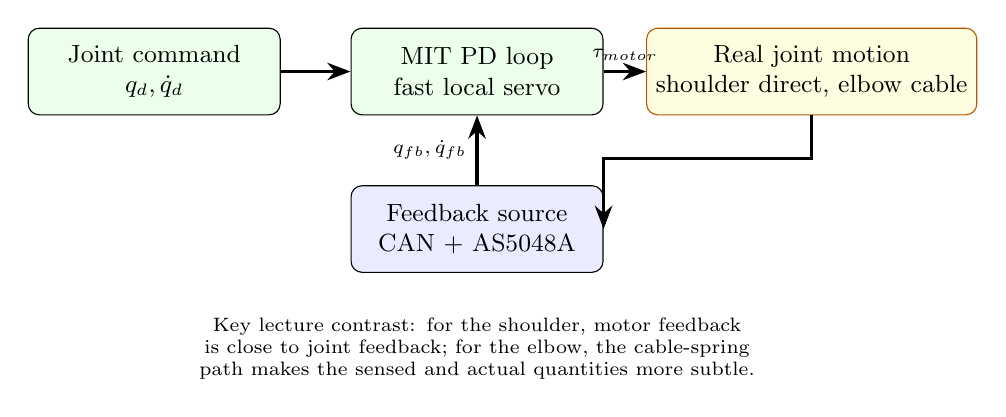
\begin{tikzpicture}[>=Stealth, every node/.style={font=\small, align=center}]
  \def\bw{3.2cm}
  \def\bh{1.1cm}

  \node[draw, rounded corners=4pt, fill=green!8,
        minimum width=\bw, minimum height=\bh] (cmd)
      at (0,0) {Joint command\\$q_d,\dot q_d$};
  \node[draw, rounded corners=4pt, fill=green!8,
        minimum width=\bw, minimum height=\bh] (mit)
      at (4.1,0) {MIT PD loop\\fast local servo};
  \node[draw, rounded corners=4pt, fill=yellow!12, draw=orange!70!black,
        minimum width=\bw, minimum height=\bh] (joint)
      at (8.35,0) {Real joint motion\\shoulder direct, elbow cable};
  \node[draw, rounded corners=4pt, fill=blue!8,
        minimum width=\bw, minimum height=\bh] (sense)
      at (4.1,-2.0) {Feedback source\\CAN + AS5048A};

  \draw[->, very thick] (cmd) -- (mit);
  \draw[->, very thick] (mit) -- node[above,font=\scriptsize] {$\tau_{motor}$} (joint);
  \draw[->, very thick] (joint.south) -- ++(0,-0.55) -| (sense.east);
  \draw[->, very thick] (sense) -- node[left,font=\scriptsize] {$q_{fb},\dot q_{fb}$} (mit);

  \node[font=\scriptsize, text width=9.8cm, below=0.45cm of sense]
      {Key lecture contrast: for the shoulder, motor feedback is close to joint feedback; for the elbow, the cable-spring path makes the sensed and actual quantities more subtle.};
\end{tikzpicture}
\caption{Phase~1 teaching visual: what the MIT PD loop is actually doing on the real arm.}
\label{fig:phase1_teaching_map}
\end{figure}

\subsection{MIT on-board PD}

The CubeMars motor implements a \textbf{proportional-derivative (PD) controller}
\emph{on the motor controller chip itself}.  Each CAN frame specifies desired angle
and gains $(K_p, K_d)$; the motor runs a closed-loop servo without host feedback.
The control law is:
\begin{equation}
  \tau_{\mathrm{motor}} = K_p(q_d - q_{\mathrm{fb}}) + K_d(\dot{q}_d - \dot{q}_{\mathrm{fb}}) + \tau_{\mathrm{ff}},
  \label{eq:mit}
\end{equation}
with $K_p\in[0,500]$ Nm/rad and $K_d\in[0,5]$ Nm$\cdot$s/rad embedded in CAN.
Setting $\tau_{\mathrm{ff}}{=}0$ gives a pure on-board spring-damper.

\subsubsection{Shoulder vs.~Elbow: What MIT Sees}

The \textbf{critical difference} is what $q_{\mathrm{fb}}$ represents:

\begin{itemize}[leftmargin=2em]
  \item \textbf{Shoulder (AK80-kv60, direct drive)}: Motor shaft rigidly bolted to joint axis.
        MIT feedback is the \emph{joint angle}~$q_1$ directly.
        Torque appears at the joint immediately.
        \vspace{0.1em}

  \item \textbf{Elbow (AK60-kv80, cable SEA)}: Motor shaft \emph{is} the DrivePulley.
        MIT feedback is the \emph{motor-side angle}~$\theta_m$ (not the joint angle~$q_2$).
        Torque must first deform the cable spring; the joint lags behind.
\end{itemize}

\subsubsection{Case 1: Direct Cable (No Spring)~--- Thought Experiment}

Imagine the elbow drive used a steel cable \textbf{without the spring inserted}
(same hardware, just remove the spring from the key-ring chain and use a solid
link instead).  Once the cable is wound taut:
\begin{equation}
  \text{(Hypothetical) } q_2 \equiv \theta_m.
  \label{eq:rigid_drive}
\end{equation}

With rigid coupling, MIT PD would act \emph{directly} on the joint:
\begin{align}
  \tau_{\mathrm{motor}} &= K_p(q_{2,d} - q_2) + K_d(\dot{q}_{2,d} - \dot{q}_2)\\[0.3em]
  &= K_p(q_{2,d} - \theta_m) + K_d(\dot{q}_{2,d} - \dot{\theta}_m)
  \label{eq:rigid_mit}
\end{align}

Joint and motor would move together ($q_2 = \theta_m$), equivalent to commanding the
joint directly.  Response would be fast and immediate.  MIT could use high gains.

\subsubsection{Case 2: Elastic Cable (With Spring)~--- Actual System}

\textbf{Without load cell:} Our elbow uses a \textbf{cable spring} with stiffness~$k_s$.  We use the
\textbf{CubeMars CAN output-shaft angle} convention throughout this subsection:
$\theta_m$ is the motor \emph{output shaft} angle reported over CAN, so there is
\textbf{no division by $N$ in the kinematics}.  The base idea is a simple torque balance:

\begin{itemize}[leftmargin=2em]
  \item $\tau_{m,\mathrm{cmd}}$: torque commanded by the MIT controller at the
        motor output shaft.
  \item $\tau_{\mathrm{spring}}$: reaction torque generated by spring stretch in the cable path.
  \item $\tau_2$: actual torque delivered to elbow joint~2.
\end{itemize}

\begin{equation}
  \tau_{m,\mathrm{cmd}} - \tau_{\mathrm{spring}} = J_{m,\mathrm{out}}\,\ddot{\theta}_m,
  \qquad
  \tau_2 = \tau_{\mathrm{spring}}.
  \label{eq:sea_torque_balance}
\end{equation}

That is, the motor output-shaft torque first accelerates the motor inertia and the
remaining transmitted torque appears at the joint through the spring.  The spring torque
comes from cable deflection:
\begin{equation}
  \delta = \rp(\theta_m - q_2), \quad
  F_{\mathrm{cable}} = k_s\,\delta + b_c\,\dot{\delta}, \quad
  \tau_{\mathrm{spring}} = \tau_2 = \rp\,F_{\mathrm{cable}}.
  \label{eq:sea_recap}
\end{equation}

\textbf{With load cell:} If an in-line \textbf{load cell} is added to the cable, then the structure of the SEA
equations does not change, but the force term becomes \emph{measured} rather than
purely inferred from the spring model.  In that case one may write
\begin{equation}
  F_{\mathrm{cable}} \approx F_{\mathrm{meas}},
  \qquad
  \tau_{\mathrm{spring}} = \tau_2 = \rp\,F_{\mathrm{meas}}.
  \label{eq:sea_loadcell}
\end{equation}
The spring relation $F_{\mathrm{cable}} = k_s\delta + b_c\dot{\delta}$ is still useful as
an internal model or consistency check, but it is no longer the only source of force
information.  This improves observability of preload, slack, friction, and hysteresis.
However, it does \emph{not} create a new direct actuator input: the controller still
commands only $\tau_{m,\mathrm{cmd}}$, while $\delta$, $F_{\mathrm{cable}}$, and
$\tau_2$ remain internal states or measured outputs of the coupled motor--spring--joint
system.

Substituting this spring torque into the motor and joint equations gives the full 2nd-order dynamics:
\begin{align}
  J_{m,\mathrm{out}}\,\ddot{\theta}_m &= \tau_{m,\mathrm{cmd}} - \rp\,F_{\mathrm{cable}}
  \quad\text{(motor output shaft)}\label{eq:motor_with_spring}\\[0.3em]
  M(q_2)\,\ddot{q}_2 + h(q_2,\dot{q}_2) &= \rp\,F_{\mathrm{cable}} \quad\text{(joint)}\label{eq:joint_with_spring}
\end{align}

where the MIT controller generates
\begin{equation}
  \tau_{m,\mathrm{cmd}} = K_p(q_{2,d} - \theta_m) + K_d(\dot{q}_{2,d} - \dot{\theta}_m).
  \label{eq:tau_m_cmd}
\end{equation}
So the CubeMars command flows to the elbow joint through the SEA in the following order:
\begin{equation}
  \tau_{m,\mathrm{cmd}}
  \;\longrightarrow\;
  \ddot{\theta}_m,\,\theta_m
  \;\longrightarrow\;
  \delta = \rp(\theta_m-q_2)
  \;\longrightarrow\;
  F_{\mathrm{cable}}
  \;\longrightarrow\;
  \tau_2 = \rp F_{\mathrm{cable}}
  \;\longrightarrow\;
  q_2.
  \label{eq:sea_signal_flow}
\end{equation}

Here $J_{m,\mathrm{out}}$ is the motor inertia reflected to the output shaft.
Equivalently, one may write the same equation in rotor-side variables using
$\theta_r = N\theta_m$, but then the spring term and torque command both carry
factors of $1/N$.  We avoid that mixed convention here because the hardware gives
$\theta_m$ directly via CAN.

MIT PD acts on motor position, not joint position.  The spring creates \emph{time lag}.
If $K_p$ is too high, the motor output shaft overshoots, stretches the spring, and stores
elastic energy before the joint catches up.  The spring then releases that energy back into
the motor-joint pair---causing \textbf{cable resonance} (underdamped oscillation).

\begin{resultbox}
\textbf{Why the spring limits gain:}
MIT closes the loop on motor position~$\theta_m$, not joint position~$q_2$.
High $K_p$ forces the motor output shaft to accelerate aggressively, straining the spring.
The spring then resists and feeds energy back into the motor-joint pair, oscillating the
system around equilibrium.
The maximum stable $K_p \approx 0.5\,k_s\,r_p^2$ (order-of-magnitude).
We use $K_p \le 30$ to stay well clear of this threshold.
\end{resultbox}

\paragraph{Gain selection without model.}
\begin{itemize}[leftmargin=2em]
  \item Start conservative: $K_p{=}20$, $K_d{=}0.5$ for both joints.
  \item Increase $K_p$ in steps of~5 until joint tracks a step command.
  \item Increase $K_d$ until oscillations are damped (typically
        $K_d \approx 0.05\sqrt{K_p}$ is a safe starting rule).
  \item Shoulder (AK80-kv60, \textbf{direct drive}): higher effective inertia;
        can tolerate $K_p$ up to~60 before feeling stiff.
  \item Elbow (AK60-kv60, \textbf{cable SEA}): the on-board MIT PD command
        goes to the \emph{motor} drum.  The MIT $K_p$ acts on motor position
        $\theta_m$, not the joint.  Keep $K_p\le 30$ to avoid exciting cable
        resonance (the spring $k_s$ limits torque bandwidth).
\end{itemize}

\begin{lstlisting}[caption={Phase~1 gain selection and MIT PD for both joints.}]
# Phase-1 gains (no model, tune empirically)
KP_SHOULDER, KD_SHOULDER = 40.0, 1.2   # AK80-kv60 shoulder
KP_ELBOW,    KD_ELBOW    = 25.0, 0.8   # AK60-kv80 elbow (cable -> lower Kp)

# On-board MIT PD (tau_ff = 0): each motor closes its own loop
shoulder.write("goal_position", {"shoulder": q_d[0]},
               kp=KP_SHOULDER, kd=KD_SHOULDER)
elbow.write(   "goal_position", {"elbow":    q_d[1]},
               kp=KP_ELBOW,    kd=KD_ELBOW)
\end{lstlisting}

\subsection{AS5048A encoder as elbow angle source}

The AS5048A is a \textbf{14-bit absolute magnetic encoder}.
Register \texttt{0x3FFF} returns the angle already corrected by the chip's
OTP zero-offset register, so \texttt{read\_angle\_rad()} gives the
correct joint angle on \emph{every} power-up with no host-side software
compensation.
\begin{equation}
  q_2^{\mathrm{enc}} = \mathrm{counts} \cdot \frac{2\pi}{2^{14}}
  \qquad (\text{zero already in chip OTP}).
  \label{eq:enc}
\end{equation}

\begin{lstlisting}[caption={AS5048A --- absolute angle read (no offset arithmetic needed).}]
from encoder_config import AS5048AConfig
from as5048a import AS5048A

enc = AS5048A(AS5048AConfig(bus=0, device=0, max_hz=1_000_000))

with enc:
    q2 = enc.read_angle_rad()   # [0, 2*pi), absolute, zero-corrected by chip
    # That's it.  No offset subtraction required after OTP is burned.
\end{lstlisting}

\paragraph{One-time OTP commissioning (done once, irreversible).}
Before running any control, mount the encoder and move the elbow to the
mechanical zero ($q_2{=}0$, arm fully extended), then burn the zero permanently:
\begin{lstlisting}[caption={One-time OTP zero burn.  Do NOT repeat -- fuses are blown permanently.}]
with AS5048A(AS5048AConfig()) as enc:
    raw = enc.set_zero(burn_otp=True)   # <<< ONE TIME ONLY
    print(f"Zero burned.  Mechanical angle latched: {raw} counts")
\end{lstlisting}
After this, \texttt{read\_angle\_rad()} on every subsequent power-up
returns the joint angle directly.  There is no need to move to a home
position or call any zeroing function.

\begin{warnbox}
  \textbf{\texttt{set\_zero(burn\_otp=False)}} writes the zero offset to
  \textbf{chip RAM} only and is \emph{lost on power cycle}.
  Always use \texttt{burn\_otp=True} for permanent commissioning.
  If the OTP is already burned, do \emph{not} call
  \texttt{set\_zero} again --- the fuse can only be programmed once.
\end{warnbox}

\paragraph{Encoder vs.\ CAN comparison check.}
At rest (no cable tension), $|q_2^{\mathrm{enc}} - q_2^{\mathrm{CAN}}|$
should be $<0.5^\circ$.  Larger offset at rest indicates a wiring or
zero-calibration error.  Offset growing with applied torque is normal
(cable spring extension) and confirms the SEA model is relevant.

\subsection{Complete Phase~1 control loop (Arm Only)}

\begin{lstlisting}[caption={Phase~1 arm-only loop: MIT PD for shoulder + elbow, no model.}]
import time
import numpy as np
from cubemars.ak_v1.ak_v1_bus import CubeMarsAkV1Bench
from cubemars.ak_v3.ak_v3_bus import CubeMarsAkV3Bench
from as5048a import AS5048A
from motor_config import (
    CubeMarsAkV1BusConfig, CubeMarsAkV1MotorConfig,
    CubeMarsAkV3BusConfig, CubeMarsMotorConfig,
)
from encoder_config import AS5048AConfig

# ---- Hardware objects (arm only: shoulder + elbow) ----
shoulder = CubeMarsAkV1Bench(channel="can1", can_id=0x01,
                              model="AK80-8", name="shoulder")
elbow    = CubeMarsAkV3Bench(channel="can1", can_id=0x02,
                              model="AK60-6", name="elbow")
enc = AS5048A(AS5048AConfig(bus=0, device=0))

# ---- Phase-1 PD gains (no model) ----
KP_SHOULDER, KD_SHOULDER = 40.0, 1.2
KP_ELBOW,    KD_ELBOW    = 25.0, 0.8

# ---- Slow sinusoid for initial motion verification ----
def traj_phase1(t):
    q_d = np.array([0.3*np.sin(0.3*t), 0.2*np.sin(0.5*t)])
    dqd = np.array([0.3*0.3*np.cos(0.3*t), 0.2*0.5*np.cos(0.5*t)])
    return q_d, dqd

DT = 0.01   # 100 Hz

with shoulder, elbow, enc:
    shoulder.enable()
    elbow.enable()
    t0 = time.monotonic()
    try:
        while True:
            t = time.monotonic() - t0
            # --- Read state (encoder gives joint angle directly) ---
            q2_enc      = enc.read_angle_rad()               # AS5048A absolute
            q1, dq1, _  = shoulder.read_state()["shoulder"]  # CAN (direct drive)
            _,  dq2, _  = elbow.read_state()["elbow"]       # CAN velocity only

            # --- Reference ---
            q_d, dqd = traj_phase1(t)

            # --- MIT on-board PD (tau_ff = 0) ---
            shoulder.write("goal_position", {"shoulder": q_d[0]},
                           kp=KP_SHOULDER, kd=KD_SHOULDER)
            elbow.write(   "goal_position", {"elbow":    q_d[1]},
                           kp=KP_ELBOW,    kd=KD_ELBOW)

            time.sleep(max(0.0, DT - (time.monotonic() - t0 - t)))

    except KeyboardInterrupt:
        print("Stopping -- zeroing all torques")
    finally:
        shoulder.write("goal_torque", {"shoulder": 0.0})
        elbow.write(   "goal_torque", {"elbow":    0.0})
\end{lstlisting}

\subsection{Phase~1 commissioning checklist}

\begin{enumerate}[leftmargin=2em]
  \item \textbf{Encoder zero (OTP) --- done once only.}  Move elbow to
        mechanical zero ($q_2{=}0$), run
        \texttt{enc.set\_zero(burn\_otp=True)}.  Never repeat.
        Afterwards \texttt{read\_angle\_rad()} always returns the correct
        joint angle with no further setup.
  \item \textbf{Direction check}: command $q_1{=}+0.1$\,rad; verify shoulder
        moves in positive direction.  Flip sign if reversed.
  \item \textbf{Encoder agree}: compare $q_2^{\mathrm{CAN}}$ with
        $q_2^{\mathrm{enc}}$ at rest ($<0.5^\circ$ expected).
        Under load the CAN angle will lag the encoder by
        $\delta/r_p$ (spring deflection) --- this is expected and correct.
        The encoder is ground truth; use it as $q_2$ in the controller.
  \item \textbf{Gain sweep}: run slow-sine trajectory; increase $K_p$ in
        steps of~5 until tracking error $<5^\circ$.
  \item \textbf{E-stop test}: Ctrl+C -- both arm motors coast to zero
        within one loop tick.
\end{enumerate}

% =========================================================================
\section{Phase 2 --- Manipulator Only (Computed Torque)}
\label{sec:phase2}
% =========================================================================

\begin{phase2box}{When to use (arm only)}
After link masses ($m_1$, $m_2$) and CoM distances ($l_{c1}$, $l_{c2}$)
are measured, the Computed-Torque (CT) law inverts the full nonlinear
dynamics, cancelling inertia and Coriolis coupling exactly.
Gravity is negligible (arm moves in the horizontal $XY$ plane; $\vg(\vq)=\mathbf{0}$).
The closed-loop error dynamics become a linear second-order system
at the design bandwidth $\omega_n$.
\textbf{Run this with shoulder + elbow only; no exo yet.}
\end{phase2box}

\begin{lecturebox}
\begin{itemize}[leftmargin=1.5em]
  \item \textbf{Teaching point 1:} Phase~2 is not a different robot; it is the same robot with a better model.
  \item \textbf{Teaching point 2:} The model parameters come from measurement plus CAD, not from guessing the final matrices directly.
  \item \textbf{Teaching point 3:} CT improves tracking by cancelling inertia and coupling before the PD terms act.
  \item \textbf{Teaching point 4:} SEA compensation and inner damping are practical fixes for what the ideal CT derivation does not capture.
\end{itemize}
\end{lecturebox}

\begin{figure}[H]
\centering
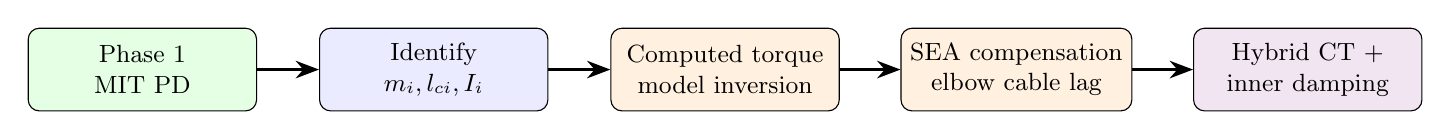
\begin{tikzpicture}[>=Stealth, every node/.style={font=\small, align=center}]
  \def\bw{2.9cm}
  \def\bh{1.05cm}

  \node[draw, rounded corners=4pt, fill=green!10,
        minimum width=\bw, minimum height=\bh] (pd)
      at (0,0) {Phase 1\\MIT PD};
  \node[draw, rounded corners=4pt, fill=blue!8,
        minimum width=\bw, minimum height=\bh] (id)
      at (3.7,0) {Identify\\$m_i,l_{ci},I_i$};
  \node[draw, rounded corners=4pt, fill=orange!12,
        minimum width=\bw, minimum height=\bh] (ct)
      at (7.4,0) {Computed torque\\model inversion};
  \node[draw, rounded corners=4pt, fill=orange!12,
        minimum width=\bw, minimum height=\bh] (sea)
      at (11.1,0) {SEA compensation\\elbow cable lag};
  \node[draw, rounded corners=4pt, fill=violet!10,
        minimum width=\bw, minimum height=\bh] (hyb)
      at (14.8,0) {Hybrid CT +\\inner damping};

  \draw[->, very thick] (pd) -- (id);
  \draw[->, very thick] (id) -- (ct);
  \draw[->, very thick] (ct) -- (sea);
  \draw[->, very thick] (sea) -- (hyb);
\end{tikzpicture}
\caption{Controller progression to discuss in lecture: each stage solves a real limitation exposed by the previous one.}
\label{fig:controller_progression_map}
\end{figure}

\subsection{Parameter identification workflow}

\begin{center}\small
\begin{tabular}{lll}
\toprule
\textbf{Parameter} & \textbf{Method} & \textbf{Units} \\
\midrule
$m_1, m_2$       & Weigh links (with motors attached) on a scale & kg \\
$l_{c1}, l_{c2}$ & Balance-point measurement or CAD export & m \\
$I_1, I_2$ (moments of inertia) & Uniform rod: $I_i{=}m_i L_i^2/3$; or CAD & kg$\cdot$m$^2$ \\
$\rp$            & Calliper measurement of drive pulley OD & m \\
$\ks$            & Static force-extension test on cable & N/m \\
\bottomrule
\end{tabular}
\end{center}

\textbf{Quick swing test:} lock the shoulder, give the elbow a small impulse
and measure the free-oscillation frequency $\omega_{\mathrm{osc}}$ (using the
AS5048A encoder).  Then $I_2 = k_{\mathrm{spring}}\,/\,\omega_{\mathrm{osc}}^2$
where $k_{\mathrm{spring}}$ is a known torsional restoring stiffness applied
via the exo cable.  (The standard pendulum formula $m_2 l_{c2} = I_2\,\omega^2/g$
does \textbf{not} apply here: gravity acts in $-Z$, perpendicular to the plane,
and contributes no restoring torque.)

\subsection{Why the CT law has this form}

The goal is to make the actual joint motion $\vq(t)$ follow a commanded
trajectory $\vq_d(t)$ as closely as possible.

Start by defining the tracking error:
\begin{equation}
  \vq_e = \vq_d - \vq, \qquad
  \vqd_e = \vqd_d - \vqd, \qquad
  \vqdd_e = \vqdd_d - \vqdd.
\end{equation}
If we could directly command joint acceleration, we would ask for the error to
obey a simple linear second-order system,
\begin{equation}
  \vqdd_e + \Kd\,\vqd_e + \Kp\,\vq_e = \mathbf{0}.
  \label{eq:ct_target_error_dyn}
\end{equation}
We choose a second-order error model because the robot itself is a
second-order mechanical system: torque affects acceleration, acceleration
changes velocity, and velocity changes position.  This form is also the
simplest one that lets us shape both tracking speed and damping through
$\Kp$ and $\Kd$.
Rearranging \eqref{eq:ct_target_error_dyn} gives the acceleration we would like
the robot to have:
\begin{equation}
  \vqdd = \vqdd_d + \Kd\,\vqd_e + \Kp\,\vq_e.
\end{equation}
This motivates the definition of the virtual input
\begin{equation}
  \bm{v} = \vqdd_d + \Kd\,\vqd_e + \Kp\,\vq_e.
  \label{eq:ct_v_choice}
\end{equation}

\paragraph{What does ``virtual input'' mean?}
The physical input to the robot is torque $\vtau$, not acceleration.  The vector
$\bm{v}$ is therefore a design quantity: it is the acceleration behavior we want
the joints to have.  The role of CT is to convert this desired acceleration
behavior into the torque required by the real nonlinear robot.

\paragraph{Small one-joint example.}
Suppose we look only at the elbow joint.  Assume the commanded motion is to hold
position, so $q_{d,2}=0.5$\,rad, $\dot{q}_{d,2}=0$, $\ddot{q}_{d,2}=0$.  If the
actual elbow state is $q_2=0.4$\,rad and $\dot{q}_2=-0.2$\,rad/s, then
\begin{equation}
  e_2 = q_{d,2}-q_2 = 0.1, \qquad
  \dot{e}_2 = \dot{q}_{d,2}-\dot{q}_2 = 0.2.
\end{equation}
With $K_{p,2}=100$ and $K_{d,2}=20$, the corresponding virtual input is
\begin{equation}
  v_2 = \ddot{q}_{d,2} + K_{d,2}\dot{e}_2 + K_{p,2}e_2
      = 0 + 20(0.2) + 100(0.1) = 14\ \text{rad/s}^2.
\end{equation}
So the controller would like the elbow to accelerate in the positive direction
at $14$\,rad/s$^2$.

Now introduce the \emph{true} manipulator dynamics:
\begin{equation}
  \M(\vq)\,\vqdd + \Cor(\vq,\vqd)\,\vqd + \vg(\vq) = \vtau.
  \label{eq:ct_start}
\end{equation}
For this arm, motion is in the horizontal $XY$ plane, so gravity produces no
joint torque and $\vg(\vq)=\mathbf{0}$.  The main nonlinear terms are therefore
the inertia matrix $\M(\vq)$ and the Coriolis term $\Cor(\vq,\vqd)\,\vqd$.

In practice, we do not know the exact model.  We instead use a predicted model
from CAD, measurements, and identification:
\begin{equation}
  \tilde{\M}(\vq), \qquad \tilde{\Cor}(\vq,\vqd), \qquad \tilde{\vg}(\vq).
\end{equation}
The practical CT law therefore commands torque using the predicted model:
\begin{equation}
  \vtau = \tilde{\M}(\vq)\,\bm{v}
        + \tilde{\Cor}(\vq,\vqd)\,\vqd
        + \tilde{\vg}(\vq).
  \label{eq:ct_model_based}
\end{equation}
This is an \emph{approximate cancellation} law: it tries to cancel the plant's
nonlinear terms using $\tilde{\M}, \tilde{\Cor}, \tilde{\vg}$, even though these
do not perfectly match the true dynamics.

Substituting \eqref{eq:ct_model_based} into \eqref{eq:ct_start} gives
\begin{equation}
  \M(\vq)\,\vqdd + \Cor(\vq,\vqd)\,\vqd + \vg(\vq)
  = \tilde{\M}(\vq)\,\bm{v} + \tilde{\Cor}(\vq,\vqd)\,\vqd + \tilde{\vg}(\vq).
  \label{eq:ct_substituted}
\end{equation}
or, after rearranging,
\begin{equation}
  \M(\vq)\,\vqdd
  = \tilde{\M}(\vq)\,\bm{v}
  + \bigl(\tilde{\Cor}(\vq,\vqd)-\Cor(\vq,\vqd)\bigr)\,\vqd
  + \bigl(\tilde{\vg}(\vq)-\vg(\vq)\bigr).
  \label{eq:ct_rearranged}
\end{equation}
This equation shows the practical case clearly: when the predicted and true
models do not match, cancellation is incomplete.  CT still helps, but the
remaining mismatch terms act like disturbances.

Only in the ideal matched-model case,
\begin{equation}
  \tilde{\M}(\vq)=\M(\vq), \qquad
  \tilde{\Cor}(\vq,\vqd)=\Cor(\vq,\vqd), \qquad
  \tilde{\vg}(\vq)=\vg(\vq),
  \label{eq:ct_exact_model}
\end{equation}
does the cancellation become exact.  Then \eqref{eq:ct_rearranged} reduces to
\begin{equation}
  \M(\vq)\,\vqdd = \M(\vq)\,\bm{v}
  \qquad \Longrightarrow \qquad
  \vqdd = \bm{v},
  \label{eq:ct_double_integrator}
\end{equation}
assuming $\M(\vq)$ is invertible.  In that ideal case the nonlinear robot is
converted into a set of double integrators.

Substituting \eqref{eq:ct_v_choice} into \eqref{eq:ct_double_integrator} gives
\begin{equation}
  \vqdd = \vqdd_d + \Kd\,\vqd_e + \Kp\,\vq_e.
\end{equation}
Using $\vqdd_e = \vqdd_d - \vqdd$ then yields
\begin{equation}
  \vqdd_e + \Kd\,\vqd_e + \Kp\,\vq_e = \mathbf{0}.
  \label{eq:ct_error_dyn}
\end{equation}
So CT is designed in two steps: first choose the acceleration behavior needed
for tracking, and then use the model to realize that behavior through torque.
In the real robot this cancellation is only approximate, which is why good
parameter identification matters and why very large $\omega_n$ can amplify
modelling errors and excite the SEA compliance at the elbow.

\subsection{Computed Torque Control law}

\begin{equation}
  \boxed{
    \vtau = \M(\vq)\bigl[\vqdd_d + \Kd\,\ved + \Kp\,\ve\bigr]
          + \Cor(\vq,\vqd)\,\vqd + \underbrace{\vg(\vq)}_{=\,\mathbf{0}}
  }
  \label{eq:ctc}
\end{equation}
where $\ve{=}\vq_d{-}\vq$, $\ved{=}\vqd_d{-}\vqd$, and
$\vg(\vq)=\mathbf{0}$ because the arm moves in the horizontal $XY$ plane
(gravity acts in $-Z$, perpendicular to the plane of motion).
Substituting into~\eqref{eq:eom} gives linear error dynamics:
$\vqdd_e + \Kd\vqd_e + \Kp\vq_e = \mathbf{0}$.
Choose $\Kp{=}\omega_n^2\mathbf{I}$, $\Kd{=}2\omega_n\mathbf{I}$
(critically damped at bandwidth $\omega_n$).

\begin{figure}[H]
\centering
\resizebox{\linewidth}{!}{%
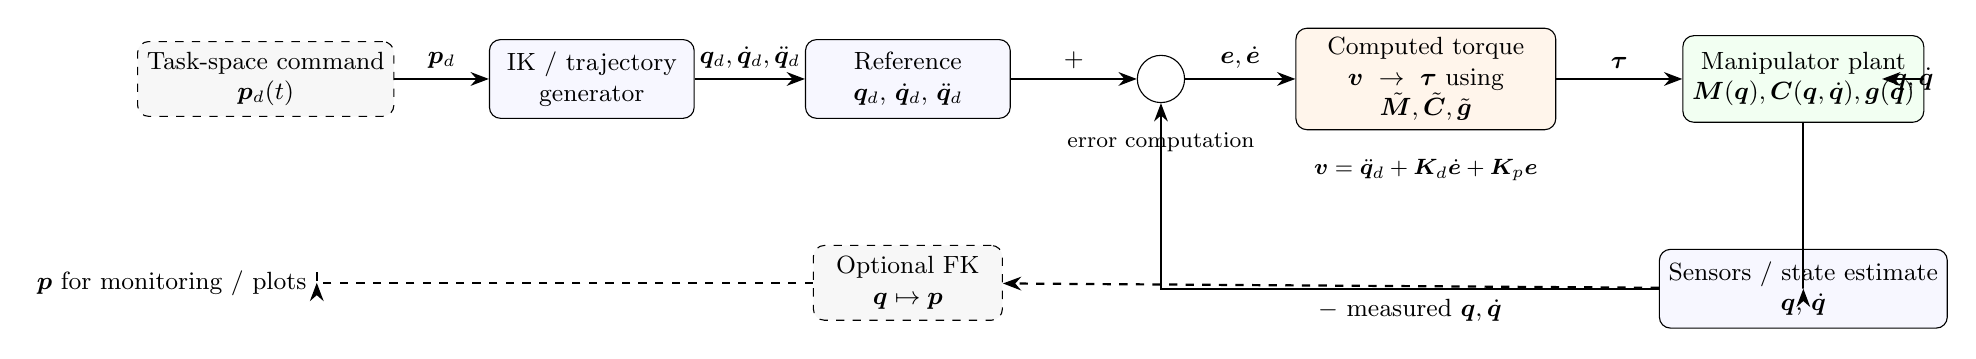
\begin{tikzpicture}[
  >=Stealth,
  every node/.style={font=\small, align=center},
  block/.style={draw, rounded corners, minimum height=1.0cm, minimum width=2.6cm, fill=blue!3},
  cblock/.style={draw, rounded corners, minimum height=1.1cm, minimum width=3.3cm, fill=orange!8},
  pblock/.style={draw, rounded corners, minimum height=1.1cm, minimum width=3.0cm, fill=green!5},
  oblock/.style={draw, dashed, rounded corners, minimum height=0.95cm, minimum width=2.4cm, fill=gray!6},
  sum/.style={draw, circle, inner sep=0pt, minimum size=6mm},
  arr/.style={-Stealth, thick},
  darr/.style={-Stealth, thick, dashed}
]
  \node[oblock] (task) {Task-space command\\$\vp_d(t)$};
  \node[block, right=1.2cm of task] (ik) {IK / trajectory\\generator};
  \node[block, right=1.4cm of ik] (qref) {Reference\\$\vq_d,\,\vqd_d,\,\vqdd_d$};
  \node[sum, right=1.6cm of qref] (sum1) {};
  \node[cblock, right=1.4cm of sum1] (ct) {Computed torque\\$\bm{v}\ \to\ \vtau$ using\\$\tilde{\M},\tilde{\Cor},\tilde{\vg}$};
  \node[pblock, right=1.6cm of ct] (plant) {Manipulator plant\\$\M(\vq),\Cor(\vq,\vqd),\vg(\vq)$};
  \node[block, below=1.6cm of plant] (sense) {Sensors / state estimate\\$\vq,\,\vqd$};
  \node[oblock, below=1.6cm of qref] (fk) {Optional FK\\$\vq \mapsto \vp$};

  \draw[arr] (task) -- node[above] {$\vp_d$} (ik);
  \draw[arr] (ik) -- node[above] {$\vq_d,\vqd_d,\vqdd_d$} (qref);
  \draw[arr] (qref) -- node[above] {$+$} (sum1);
  \draw[arr] (sum1) -- node[above] {$\ve,\ved$} (ct);
  \draw[arr] (ct) -- node[above] {$\vtau$} (plant);
  \draw[arr] (plant) -- ++(1.0,0) node[right] {$\vq,\vqd$};
  \draw[arr] (plant) |- (sense);
  \draw[arr] (sense) -| node[pos=0.25, below] {$-$ measured $\vq,\vqd$} (sum1);
  \draw[darr] (sense) -- (fk);
  \draw[darr] (fk.west) -| ++(-6.3,0) node[left] {$\vp$ for monitoring / plots};

  \node[below=0.25cm of sum1, font=\footnotesize] {error computation};
  \node[below=0.25cm of ct, font=\footnotesize] {$\bm{v}=\vqdd_d+\Kd\ved+\Kp\ve$};
\end{tikzpicture}
}
\caption{Computed-torque control signal flow.  A task-space command can first be converted to a joint-space reference through IK, or $\vq_d(t)$ can be provided directly.  The CT block uses the predicted model to generate torque $\vtau$, the manipulator returns measured joint state $\vq,\vqd$, and an optional FK block maps the measured state back to end-effector position for monitoring.}
\label{fig:ct_block_diagram}
\end{figure}

\paragraph{Motor torque limits (Phase~2):}
\begin{center}\small
\begin{tabular}{llll}
\toprule
Motor & Model & $T_{\max}$ & Clip in code \\
\midrule
Shoulder & AK80-kv60 (V1.x) & 32\,N$\cdot$m & \texttt{np.clip(tau[0], -28, 28)} \\
Elbow    & AK60-kv80 (V3.0) & 15\,N$\cdot$m & \texttt{np.clip(tau[1], -12, 12)} \\
\bottomrule
\end{tabular}
\end{center}

\begin{lstlisting}[caption={Computed Torque implementation (Phase~2 arm).}]
import numpy as np

# ---- Parameters (fill from identification) ----
L = np.array([0.335, 0.380])   # m
m = np.array([5.313, 0.764])   # kg  (URDF; re-weigh on hardware)
g = 0.0  # horizontal XY plane: gravity acts in -Z, perpendicular to motion plane
T_MAX = np.array([28.0, 12.0]) # N.m  [shoulder, elbow]

def inertia(q):
    c2  = np.cos(q[1])
    M11 = 4/3*m[0]*L[0]**2 + m[1]*(L[0]**2+4/3*L[1]**2+2*L[0]*L[1]*c2)
    M12 = m[1]*(4/3*L[1]**2 + L[0]*L[1]*c2)
    M22 = 4/3*m[1]*L[1]**2
    return np.array([[M11, M12], [M12, M22]])

def coriolis(q, dq):
    h = -m[1]*L[0]*L[1]*np.sin(q[1])
    return np.array([[h*dq[1], h*(dq[0]+dq[1])], [-h*dq[0], 0.0]])

def gravity(q):
    # Horizontal plane: gravity acts in -Z, perpendicular to XY plane of motion.
    # No joint torque from gravity => g(q) = 0.
    return np.zeros(2)

# ---- CT gains (omega_n = 12 rad/s, critically damped) ----
wn = 12.0
Kp = wn**2 * np.eye(2)
Kd = 2*wn  * np.eye(2)

def ct_torque(q, dq, q_d, dqd, qdd_d):
    e  = q_d - q
    de = dqd - dq
    v  = qdd_d + Kd @ de + Kp @ e
    tau = inertia(q) @ v + coriolis(q, dq) @ dq + gravity(q)
    return np.clip(tau, -T_MAX, T_MAX)
\end{lstlisting}

\subsection{SEA cable compensation at the elbow}
\label{sec:sea}

The elbow is driven via a cable spring (stiffness $\ks$) between the motor
drum and the joint pulley.  The spring extension is:
\begin{equation}
  \delta = \lm - \rp\,q_2, \qquad
  \dot{\delta} = \lmd - \rp\,\dot{q}_2,
  \label{eq:delta}
\end{equation}
where $\lm{=}\rp\,\theta_m$ is the cable displacement paid out by the
drum.  The cable force and resulting joint torque are:
\begin{equation}
  F_{\mathrm{cable}} = \ks\,\delta + \bc\,\dot{\delta},\qquad
  \tau_2^{\mathrm{actual}} = \rp\,F_{\mathrm{cable}}.
  \label{eq:sea_tau}
\end{equation}

To invert this for a desired CT torque, compute the required cable displacement:
\begin{equation}
  F_{\mathrm{des}} = \frac{\tau_{2,\mathrm{des}}}{\rp}, \qquad
  \lm^{\mathrm{des}} = \rp\,q_2^{\mathrm{enc}}
                      + \frac{F_{\mathrm{des}} - \bc\,\dot{\delta}}{\ks}.
  \label{eq:sea_inv}
\end{equation}

\begin{lstlisting}[caption={SEA cable compensation for the elbow (Phase~2).}]
# SEA parameters (from cable force-extension test on hardware)
K_S = 10.0     # N/m  (measure on real cable)
B_C = 0.5      # N.s/m
R_P = 0.04775  # m  (big-pulley radius)

def sea_compensation(tau_des_2, q2_enc, dq2_enc, l_m, dl_m):
    """Convert desired elbow torque -> required cable displacement."""
    delta  = l_m  - R_P * q2_enc
    ddelta = dl_m - R_P * dq2_enc
    F_des  = tau_des_2 / R_P
    l_m_des = R_P * q2_enc + (F_des - B_C * ddelta) / K_S
    return l_m_des
\end{lstlisting}

\begin{warnbox}
\textbf{SEA bandwidth.}
Raise $\ks$ (use stiffer cable / pre-tension) or lower $\omega_n$ if
oscillatory torque tracking is observed on hardware.
\end{warnbox}

\subsection{Hybrid CT + inner MIT damping}

Send the CT output as $\tau_{\mathrm{ff}}$ and keep small on-board $K_d$
to damp encoder noise without fighting the feedforward:
\begin{equation}
  \tau_{\mathrm{ff}} = \vtau_{\mathrm{CT}},\quad
  K_p^{\mathrm{MIT}}{=}0,\quad K_d^{\mathrm{MIT}}{=}0.3\text{--}0.6.
  \label{eq:hybrid}
\end{equation}

\begin{figure}[H]
\centering
\resizebox{\linewidth}{!}{%
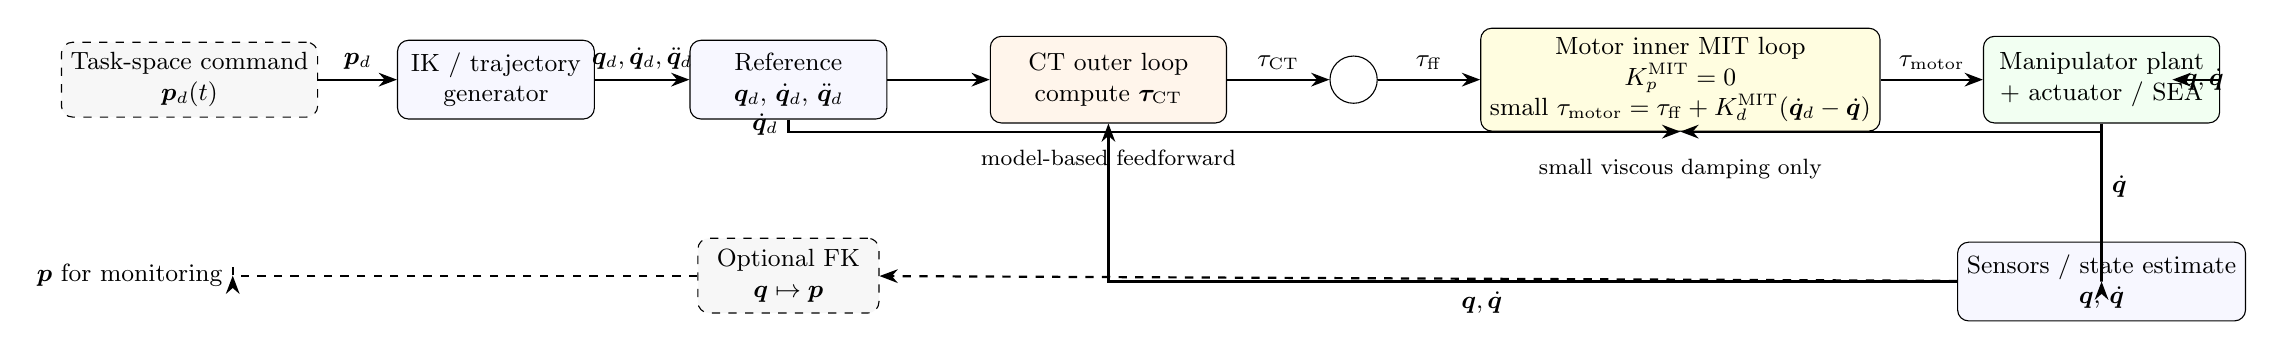
\begin{tikzpicture}[
  >=Stealth,
  every node/.style={font=\small, align=center},
  block/.style={draw, rounded corners, minimum height=1.0cm, minimum width=2.5cm, fill=blue!3},
  cblock/.style={draw, rounded corners, minimum height=1.1cm, minimum width=3.0cm, fill=orange!8},
  iblock/.style={draw, rounded corners, minimum height=1.1cm, minimum width=3.2cm, fill=yellow!12},
  pblock/.style={draw, rounded corners, minimum height=1.1cm, minimum width=3.0cm, fill=green!5},
  oblock/.style={draw, dashed, rounded corners, minimum height=0.95cm, minimum width=2.3cm, fill=gray!6},
  sum/.style={draw, circle, inner sep=0pt, minimum size=6mm},
  arr/.style={-Stealth, thick},
  darr/.style={-Stealth, thick, dashed}
]
  \node[oblock] (task) {Task-space command\\$\vp_d(t)$};
  \node[block, right=1.0cm of task] (ik) {IK / trajectory\\generator};
  \node[block, right=1.2cm of ik] (qref) {Reference\\$\vq_d,\,\vqd_d,\,\vqdd_d$};
  \node[cblock, right=1.3cm of qref] (ct) {CT outer loop\\compute $\vtau_{\mathrm{CT}}$};
  \node[sum, right=1.3cm of ct] (sumtau) {};
  \node[iblock, right=1.3cm of sumtau] (mit) {Motor inner MIT loop\\$K_p^{\mathrm{MIT}}=0$\\small $\tau_{\mathrm{motor}}=\tau_{\mathrm{ff}} + K_d^{\mathrm{MIT}}(\vqd_d-\vqd)$};
  \node[pblock, right=1.3cm of mit] (plant) {Manipulator plant\\+ actuator / SEA};
  \node[block, below=1.5cm of plant] (sense) {Sensors / state estimate\\$\vq,\,\vqd$};
  \node[oblock, below=1.5cm of qref] (fk) {Optional FK\\$\vq \mapsto \vp$};

  \draw[arr] (task) -- node[above] {$\vp_d$} (ik);
  \draw[arr] (ik) -- node[above] {$\vq_d,\vqd_d,\vqdd_d$} (qref);
  \draw[arr] (qref) -- (ct);
  \draw[arr] (qref.south) |- node[pos=0.22, left] {$\vqd_d$} (mit.south);
  \draw[arr] (ct) -- node[above] {$\tau_{\mathrm{CT}}$} (sumtau);
  \draw[arr] (sumtau) -- node[above] {$\tau_{\mathrm{ff}}$} (mit);
  \draw[arr] (mit) -- node[above] {$\tau_{\mathrm{motor}}$} (plant);
  \draw[arr] (plant) -- ++(0.9,0) node[right] {$\vq,\vqd$};
  \draw[arr] (plant) |- (sense);
  \draw[arr] (sense.west) -| node[pos=0.28, below] {$\vq,\vqd$} (ct.south);
  \draw[arr] (sense.north) |- node[pos=0.25, right] {$\vqd$} (mit.south);
  \draw[darr] (sense) -- (fk);
  \draw[darr] (fk.west) -| ++(-5.9,0) node[left] {$\vp$ for monitoring};

  \node[below=0.22cm of ct, font=\footnotesize] {model-based feedforward};
  \node[below=0.22cm of mit, font=\footnotesize] {small viscous damping only};
\end{tikzpicture}%
}
\caption{Hybrid CT signal flow.  The outer loop computes the model-based torque $\tau_{\mathrm{CT}}$, which is sent as feedforward $\tau_{\mathrm{ff}}$ to the motor's inner MIT loop.  The MIT loop does not perform position control ($K_p^{\mathrm{MIT}}=0$); it only adds local velocity damping through the term $K_d^{\mathrm{MIT}}(\vqd_d-\vqd)$, producing the final motor torque $\tau_{\mathrm{motor}}$.  The measured joint state $\vq,\vqd$ feeds back to the CT outer loop, while the measured velocity $\vqd$ and desired velocity $\vqd_d$ form the inner damping loop.  IK and FK remain optional when the command originates in task space or when end-effector motion is monitored.}
\label{fig:hybrid_ct_block_diagram}
\end{figure}

\begin{lstlisting}[caption={Hybrid CT: model feedforward + small on-board damping.}]
tau = ct_torque(q, dq, q_d, dqd, qdd_d)

# Shoulder: AK80-kv60 V1.x API
shoulder.write("mit_command", {"shoulder": q_d[0]},
               kp=0.0, kd=0.4, dq_des=dqd[0], tau_ff=tau[0])
# Elbow: AK60-kv80 V3.0 API
elbow.write("mit_command", {"elbow": q_d[1]},
            kp=0.0, kd=0.4, dq_des=dqd[1], tau_ff=tau[1])
\end{lstlisting}

\subsection{Obtaining the real model from the robot in practice}

For CT, we do not measure $\M(\vq)$, $\Cor(\vq,\vqd)$, and $\vg(\vq)$ directly as matrices.
Instead, we obtain the constant physical parameters of the arm and then build
the model from them.

\paragraph{What we actually need.}
For the 2-DOF arm, the useful quantities are
\begin{equation}
  L_1,\; L_2,\; m_1,\; m_2,\; l_{c1},\; l_{c2},\; I_1,\; I_2.
\end{equation}
Once these are available, we can construct $\M(\vq)$, $\Cor(\vq,\vqd)$, and
$\vg(\vq)$.

\paragraph{What is directly doable on the real robot?}
\begin{itemize}[leftmargin=2em]
  \item Measure $L_1$ and $L_2$ with a caliper or tape.
  \item Measure $m_1$ and $m_2$ by weighing each link assembly, including
        fasteners, brackets, adapters, and any mounted hardware that moves with
        the link.
  \item Measure pulley radius $\rp$ directly.
  \item Measure cable stiffness $\ks$ with a static force-extension test.
  \item Use CAD as the initial source for $l_{c1}$, $l_{c2}$, $I_1$, and $I_2$.
\end{itemize}

\paragraph{Recommended workflow.}
\begin{enumerate}[leftmargin=2em]
  \item Start from CAD values for CoM locations and moments of inertia.
  \item Replace CAD masses and lengths with measured hardware values.
  \item Load the resulting parameters into the robot model.
  \item If tracking is not good enough, refine the uncertain parameters using
        logged motion and torque data.
\end{enumerate}

\begin{figure}[H]
\centering
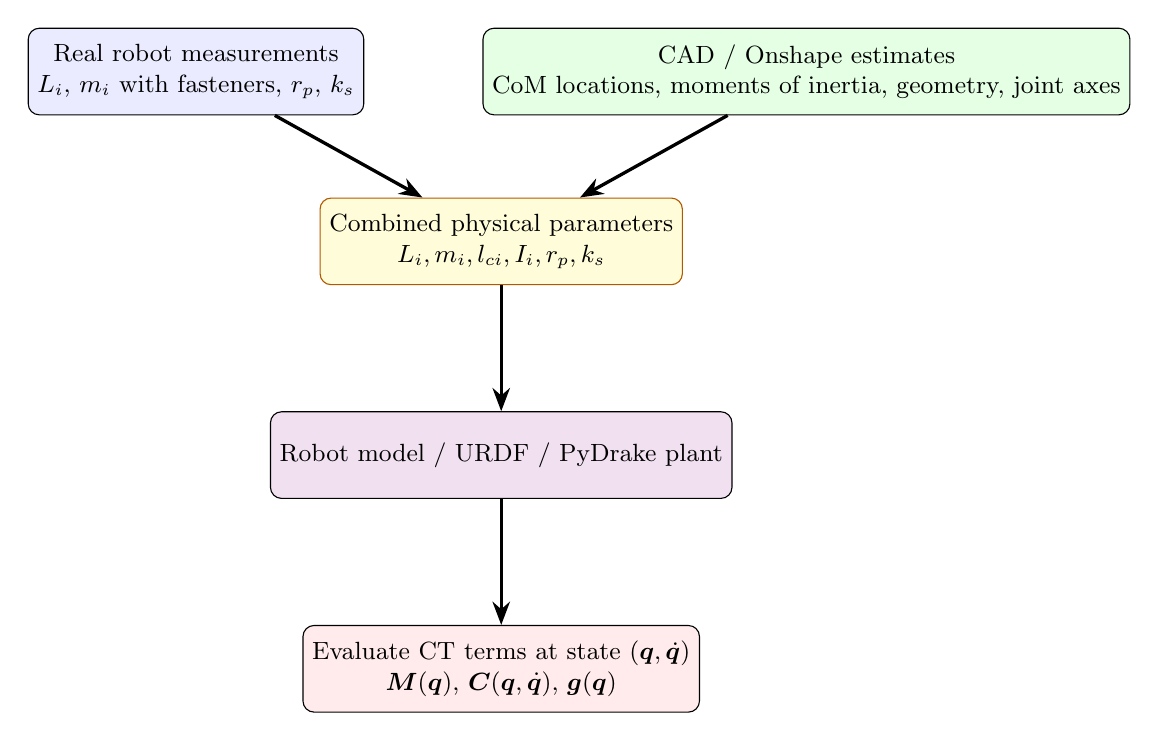
\begin{tikzpicture}[>=Stealth, node distance=1.6cm, every node/.style={font=\small, align=center}]
  \def\bw{3.2cm}
  \def\bh{1.1cm}

  \node[draw, rounded corners=4pt, fill=blue!8,
    minimum width=\bw, minimum height=\bh] (measure)
    {Real robot measurements\\$L_i$, $m_i$ with fasteners, $r_p$, $k_s$};

  \node[draw, rounded corners=4pt, fill=green!10,
    minimum width=\bw, minimum height=\bh, right=1.5cm of measure] (cad)
    {CAD / Onshape estimates\\CoM locations, moments of inertia, geometry, joint axes};

  \node[draw, rounded corners=4pt, fill=yellow!15, draw=orange!70!black,
    minimum width=3.9cm, minimum height=\bh, below=1.6cm of $(measure)!0.5!(cad)$] (params)
    {Combined physical parameters\\$L_i, m_i, l_{ci}, I_i, r_p, k_s$};

  \node[draw, rounded corners=4pt, fill=violet!12,
    minimum width=4.2cm, minimum height=\bh, below=1.6cm of params] (model)
    {Robot model / URDF / PyDrake plant};

  \node[draw, rounded corners=4pt, fill=red!8,
    minimum width=4.6cm, minimum height=\bh, below=1.6cm of model] (dyn)
    {Evaluate CT terms at state $(\vq,\vqd)$\\$\M(\vq)$, $\Cor(\vq,\vqd)$, $\vg(\vq)$};

  \draw[->, very thick] (measure) -- (params);
  \draw[->, very thick] (cad) -- (params);
  \draw[->, very thick] (params) -- (model);
  \draw[->, very thick] (model) -- (dyn);
\end{tikzpicture}
\caption{Practical flow for identifying the quantities needed to build $\M(\vq)$, $\Cor(\vq,\vqd)$, and $\vg(\vq)$. Measured link masses should include the real moving hardware attached to each link, including fasteners and brackets.}
\label{fig:identify_mcg_flow}
\end{figure}

\paragraph{What this means for $\M$, $\Cor$, and $\vg$.}
$\M(\vq)$, $\Cor(\vq,\vqd)$, and $\vg(\vq)$ are state-dependent quantities,
so they are not measured once and stored as constants.  The constants are the
physical parameters above.  After those are known, the model can be evaluated
at any joint state.

\begin{resultbox}
The practical goal is simple: measure what can be measured on the robot, take
the remaining inertial quantities from CAD, and refine only if the controller
needs better accuracy.
\end{resultbox}

\subsection{Using Onshape and PyDrake to obtain the dynamic model}

If the arm already exists in Onshape, this is the cleanest route to a usable
model for PyDrake.

\paragraph{Important distinction.}
The OBJ file is \emph{not} the dynamic model by itself.  The OBJ file mainly
stores the mesh geometry used for visualisation and collision.  The quantities
needed for dynamics --- masses, centres of mass, and inertia tensors --- must
appear in the URDF or SDF inertial tags.  PyDrake reads those inertial
properties from the robot description, not from the OBJ mesh alone.

\paragraph{What should come from CAD?}
From Onshape or CAD we should export:
\begin{itemize}[leftmargin=2em]
  \item link geometry,
  \item link masses,
  \item centre-of-mass locations,
  \item inertia tensors,
  \item joint locations and joint axes.
\end{itemize}
These inertial values must be written into the URDF.  The OBJ files are only
used as mesh assets.

\paragraph{Practical pipeline.}
\begin{equation}
  \text{Onshape/CAD}
  \;\Longrightarrow\;
  \text{URDF with inertial parameters}
  \;\Longrightarrow\;
  \text{load into PyDrake}
  \;\Longrightarrow\;
  \text{evaluate } \M(\vq)\text{ and bias terms}.
\end{equation}
In this pipeline, OBJ conversion is only a supporting step so that Drake can
load the mesh assets cleanly.

\paragraph{What does PyDrake calculate?}
Once the URDF is loaded into a \texttt{MultibodyPlant}, PyDrake can evaluate the
robot dynamics at the current joint state.  Conceptually, this means:
\begin{align}
  \M(\vq) &\leftarrow \text{mass matrix from the plant at } \vq, \\
  \vtau_{bias}(\vq,\vqd) &\leftarrow \text{bias term from the plant},
\end{align}
where the bias term contains Coriolis and centrifugal effects, and also gravity
if gravity is enabled.  In our horizontal-plane case, gravity is typically set
to zero or contributes no in-plane torque, so the bias term mainly represents
the velocity-dependent effects associated with $\Cor(\vq,\vqd)\,\vqd$.

\paragraph{What this means in practice.}
If the URDF inertial values are good, PyDrake can directly provide the dynamic
terms needed for CT.  If the CAD values are only approximate, then the Drake
model is still useful, but its accuracy is limited by the parameters stored in
the URDF.

\begin{lstlisting}[caption={Conceptual PyDrake route to obtain the dynamic terms from a URDF model.}]
plant_context = plant.CreateDefaultContext()
plant.SetPositions(plant_context, model_instance, q)
plant.SetVelocities(plant_context, model_instance, qd)

M = plant.CalcMassMatrixViaInverseDynamics(plant_context)
bias = plant.CalcBiasTerm(plant_context)

# Horizontal-plane arm: gravity contribution is zero or disabled.
# For CT, use M and bias directly in the feedforward torque calculation.
\end{lstlisting}

\begin{resultbox}
Use Onshape for geometry and inertial parameters, store them in the URDF, use
OBJ only for meshes, and let PyDrake evaluate $\M(\vq)$ and the nonlinear bias
term needed by the CT controller.
\end{resultbox}

% =========================================================================
\section{Phase 1 with Exo --- Transparent Mode}
\label{sec:phase1_exo}
% =========================================================================

\begin{phase1box}{When to add the exo}
Once the manipulator tracks reliably under Phase~1 MIT PD (arm only,
Section~\ref{sec:phase1}), mount the exosuit Damiao motors.  In
\emph{transparent} mode they follow the elbow encoder angle so the cables
stay slack and the arm experiences no additional loading.  This step
verifies correct exo motor direction and cable routing before activating
co-contraction in Phase~2 with Exo.
\end{phase1box}

\subsection{Exo Damiao motors --- transparent mode}

The Damiao motor follows the elbow encoder angle with \emph{zero} cable
tension so it does not load the arm:
\begin{equation}
  \tau_{\mathrm{exo}} = 0,\quad
  q_{d,\mathrm{exo}} = +q_2^{\mathrm{enc}},\quad
  K_p^{\mathrm{exo}} = 0.
  \label{eq:exo_transparent}
\end{equation}

\begin{lstlisting}[caption={Exo transparent mode: Damiao motor follows AS5048A encoder.}]
# Read true elbow angle from absolute encoder
q2_enc = enc.read_angle_rad()

# Exo motor tracks joint angle -> zero cable extension -> zero torque
exo.write("mit_command",
          {"exo":  q2_enc},
          kp=0.0, kd=0.05, tau_ff=0.0)   # light viscous damp only
\end{lstlisting}

\begin{warnbox}
\textbf{Exo motor direction.}
Verify sign convention with slow manual elbow flexion before running the
full loop: the cable should remain slack (no resistance felt by hand).
\end{warnbox}

\subsection{Complete 4-actuator Phase~1 loop (arm + transparent exo)}

\begin{lstlisting}[caption={4-actuator Phase~1 loop: MIT PD + transparent exo.}]
import time
import numpy as np
from cubemars.ak_v1.ak_v1_bus import CubeMarsAkV1Bench
from cubemars.ak_v3.ak_v3_bus import CubeMarsAkV3Bench
from damiao.damiao_bus import DamiaoBus
from as5048a import AS5048A
from motor_config import (
    CubeMarsAkV1BusConfig, CubeMarsAkV1MotorConfig,
    CubeMarsAkV3BusConfig, CubeMarsMotorConfig,
    DamiaoBusConfig, DamiaoMotorConfig,
)
from encoder_config import AS5048AConfig

# ---- Hardware objects ----
shoulder = CubeMarsAkV1Bench(channel="can1", can_id=0x01,
                              model="AK80-8", name="shoulder")
elbow    = CubeMarsAkV3Bench(channel="can1", can_id=0x02,
                              model="AK60-6", name="elbow")
exo      = DamiaoBus(DamiaoBusConfig(
    port="/dev/ttyACM0",
    motors={"exo": DamiaoMotorConfig(can_id=0x01)},
))
enc = AS5048A(AS5048AConfig(bus=0, device=0))

# ---- Phase-1 PD gains (no model) ----
KP_SHOULDER, KD_SHOULDER = 40.0, 1.2
KP_ELBOW,    KD_ELBOW    = 25.0, 0.8

def traj_phase1(t):
    q_d = np.array([0.3*np.sin(0.3*t), 0.2*np.sin(0.5*t)])
    dqd = np.array([0.3*0.3*np.cos(0.3*t), 0.2*0.5*np.cos(0.5*t)])
    return q_d, dqd

DT = 0.01   # 100 Hz

with shoulder, elbow, exo, enc:
    shoulder.enable()
    elbow.enable()
    exo.connect()
    t0 = time.monotonic()
    try:
        while True:
            t = time.monotonic() - t0
            q2_enc      = enc.read_angle_rad()
            q1, dq1, _  = shoulder.read_state()["shoulder"]
            _,  dq2, _  = elbow.read_state()["elbow"]
            q_d, dqd = traj_phase1(t)

            shoulder.write("goal_position", {"shoulder": q_d[0]},
                           kp=KP_SHOULDER, kd=KD_SHOULDER)
            elbow.write(   "goal_position", {"elbow":    q_d[1]},
                           kp=KP_ELBOW,    kd=KD_ELBOW)

            # --- Exo transparent: follow joint angle, zero torque ---
            exo.write("mit_command",
                      {"exo":  q2_enc},
                      kp=0.0, kd=0.05, tau_ff=0.0)

            time.sleep(max(0.0, DT - (time.monotonic() - t0 - t)))

    except KeyboardInterrupt:
        print("Stopping -- zeroing all torques")
    finally:
        shoulder.write("goal_torque", {"shoulder": 0.0})
        elbow.write(   "goal_torque", {"elbow":    0.0})
        exo.write("goal_torque", {"exo": 0.0})
\end{lstlisting}

\subsection{Exo transparent commissioning checklist}

\begin{enumerate}[leftmargin=2em]
  \item \textbf{Exo transparent check}: manually flex the elbow through its full
        range of motion --- no resistance should be felt from the exo cable.
  \item \textbf{Direction check}: if resistance is felt in either direction,
        reverse the exo motor direction mapping and repeat.
  \item \textbf{Cable slack at rest}: at zero velocity, verify cable tension
        reads near zero (compare exo encoder to AS5048A encoder).
  \item \textbf{E-stop test}: Ctrl+C -- all four motors coast to zero
        within one loop tick.
\end{enumerate}

% =========================================================================
\section{Phase 2 with Exo --- CT + Co-contraction}
\label{sec:phase2_exo}
% =========================================================================

\begin{phase2box}{When to add the exo}
Once the arm tracks reliably under Phase~2 CT (arm only,
Section~\ref{sec:phase2}), activate the exo Damiao motors.
First confirm the transparent baseline from Section~\ref{sec:phase1_exo},
then switch to co-contraction mode by commanding a symmetric angular
offset $\Delta\theta$ on both exo cables.  This adds programmable
joint-level stiffness $K_e$ at the elbow without changing the CT controller.
\end{phase2box}

\subsection{Exo co-contraction activation}

The exo Damiao motors are commanded with a symmetric offset so that both
cables develop equal pretension, adding co-contraction stiffness $K_e$ at
the elbow
(\texttt{Exo\_Impedance\_Learning\_PyDrake\_Implementation.tex}):
\begin{equation}
  \frac{\theta_{mR}}{N} \to q_{2,\mathrm{des}} + \Delta\theta, \qquad
  \frac{\theta_{mL}}{N} \to -q_{2,\mathrm{des}} + \Delta\theta,
  \label{eq:exo_cmd}
\end{equation}
where $\Delta\theta$ is the co-contraction offset [rad].  The effective
joint stiffness is approximately $K_e \approx 2\,\ks^{\mathrm{exo}}\,\rp^2$.

\begin{lstlisting}[caption={Exo co-contraction activation (Phase~2 with exo).}]
DELTA_THETA = 0.10    # rad  (co-contraction offset; tune empirically)
EXO_KP = 2.0;  EXO_KD = 0.1

def exo_command(q2_des, activate, dth=DELTA_THETA):
    if activate:
        return q2_des + dth,  -q2_des + dth
    else:
        return q2_des,        -q2_des     # transparent

q2_des_exo = q_d[1]     # CT desired elbow angle
th_R, th_L = exo_command(q2_des_exo, activate=exo_on)
exo.write("mit_command",
          {"exo_r": th_R, "exo_l": th_L},
          kp=EXO_KP, kd=EXO_KD, tau_ff=0.0)
\end{lstlisting}

% =========================================================================
\section{Trajectory Generation}
\label{sec:traj}
% =========================================================================

\subsection{Minimum-jerk point-to-point}

\begin{equation}
  \vp_d(t) = \vp_0 + (\vp_f{-}\vp_0)
    \bigl[10(t/T)^3 - 15(t/T)^4 + 6(t/T)^5\bigr].
  \label{eq:minjerk}
\end{equation}

\subsection{Circle trajectory}

Matches \texttt{CircleTrajectory} in \texttt{controller/trajectory\_drake.py}:

\begin{lstlisting}[caption={Circle trajectory + IK for hardware.}]
import numpy as np

def circle(t, center=np.array([0.40,0.20]), r=0.05, T=4.0):
    th  = 2*np.pi*t/T
    p   = center + r*np.array([np.cos(th),   np.sin(th)])
    pd  =          r*2*np.pi/T*np.array([-np.sin(th),  np.cos(th)])
    pdd = -r*(2*np.pi/T)**2*np.array([np.cos(th), np.sin(th)])
    return p, pd, pdd

def ik(p, L):
    D   = np.clip((p@p-L[0]**2-L[1]**2)/(2*L[0]*L[1]), -1+1e-6, 1-1e-6)
    q2  = np.arctan2(np.sqrt(1-D**2), D)
    q1  = np.arctan2(p[1],p[0]) - np.arctan2(L[1]*np.sin(q2),
                                               L[0]+L[1]*np.cos(q2))
    return np.array([q1, q2])

def jacobian(q, L):
    s12 = np.sin(q[0]+q[1]); c12 = np.cos(q[0]+q[1])
    return np.array([[-L[0]*np.sin(q[0])-L[1]*s12, -L[1]*s12],
                     [ L[0]*np.cos(q[0])+L[1]*c12,  L[1]*c12]])
\end{lstlisting}

% =========================================================================
\section{Controller Comparison}
\label{sec:compare}
% =========================================================================

\begin{center}\small
\begin{tabular}{p{3.2cm} p{2.2cm} p{1.6cm} p{2.4cm} p{3.2cm}}
\toprule
\textbf{Controller} & \textbf{Model needed} & \textbf{Phase} & \textbf{Steady-state} & \textbf{Use case} \\
\midrule
MIT on-board PD          & None            & 1   & Gravity sag   & Commissioning, gain tuning \\
PD + gravity comp.       & $\vg$ only      & 1.5 & Eliminated    & Slow Cartesian after $m_i$ known \\
\textbf{CT (joint)}      & Full $\M,\Cor,\vg$ & 2 & Eliminated & Trajectory tracking \\
CT + SEA compensation    & Model + $\ks$   & 2   & Eliminated    & Compliant elbow cable \\
CT + exo co-contraction  & Model + $K_e$   & 2+  & Eliminated    & Exo rehab stiffness \\
Cartesian PD (J-transp.) & $\J$ + $\vg$   & 2   & Designed-in   & Safe compliant interaction \\
\bottomrule
\end{tabular}
\end{center}

% =========================================================================
\section{Safety Constraints}
\label{sec:safety}
% =========================================================================

\begin{itemize}[leftmargin=2em]
  \item \textbf{Torque limits:}
        $|\tau_1|{\le}28$\,N$\cdot$m (AK80-kv60),
        $|\tau_2|{\le}12$\,N$\cdot$m (AK60-kv80),
        $|\tau_{\mathrm{exo}}|{\le}8$\,N$\cdot$m per Damiao.
        Always \texttt{np.clip} before sending.
  \item \textbf{Velocity limits:}
        $|\dot{q}_1|{\le}30$\,rad/s, $|\dot{q}_2|{\le}45$\,rad/s.
        Saturate $\dot{q}_d$ in trajectory generator.
  \item \textbf{Workspace limits:}
        $q_1{\in}[-\pi/2,\,\pi]$, $q_2{\in}[10^\circ,\,170^\circ]$.
        Enforce in IK; reject unreachable Cartesian targets.
  \item \textbf{Encoder agreement check:}
        Each tick verify $|q_2^{\mathrm{CAN}}{-}q_2^{\mathrm{enc}}|<0.15$\,rad.
        Larger discrepancy: switch to safe-hold (MIT PD, current position,
        low gains).
  \item \textbf{Thermal:}
        Monitor MOS temperature from \texttt{read\_raw()}; pause if $>70^\circ$C.
  \item \textbf{Emergency stop:}
        On SIGINT/Ctrl+C: zero torque on all four actuators via context-manager
        \texttt{\_\_exit\_\_} in each bus class.
\end{itemize}

% =========================================================================
\section{Simulation Validation Bridge}
\label{sec:sim}
% =========================================================================

All hardware controllers are first validated in the PyDrake simulation
framework.  The controller core (\texttt{rl/computed\_torque\_controller.py})
is \textbf{engine-agnostic} (pure NumPy, no Drake imports) so the same code
runs in simulation and on hardware.

\begin{center}\small
\begin{tabular}{ll}
\toprule
\textbf{Hardware mode} & \textbf{Simulation analogue} \\
\midrule
Phase~1 MIT PD (no model) &
  \texttt{script\_...\_with\_exo\_pydrake.py} (weak $K_p$/$K_d$) \\
Phase~2 CT (arm only) &
  \texttt{Computed\_Torque\_PyDrake\_Implementation.tex} \\
Phase~2 CT + SEA &
  \texttt{SEA\_Cable\_PyDrake\_Implementation.tex}, \texttt{--sea-mode position} \\
Phase~2 CT + exo &
  \texttt{Exo\_Impedance\_Learning\_PyDrake\_Implementation.tex},
  \texttt{--exo-activate} \\
\bottomrule
\end{tabular}
\end{center}

\paragraph{Workflow.}
\begin{enumerate}[leftmargin=2em]
  \item Tune gains in PyDrake (Meshcat at \texttt{http://localhost:7000}).
  \item Export to \texttt{controller\_config.yaml}.
  \item Load YAML on Jetson Orin for hardware deployment.
  \item Compare logged trajectories with simulation via
        \texttt{compare\_exo\_pydrake\_vs\_isaac.py}.
\end{enumerate}

\end{document}
